% ===========================================================================
% BRCA Multi-Omics Data Mining — Academic Paper
% Version: 0518-1527  (ctexbook + TOC/LOF/LOT + template format)
% ===========================================================================
\documentclass[12pt,a4paper,openany]{ctexbook}

\usepackage[top=2.5cm, bottom=2.5cm, left=3cm, right=2.5cm]{geometry}
\usepackage{graphicx}
\usepackage{booktabs}
\usepackage[labelfont=bf,font=small]{caption}
\usepackage[hidelinks]{hyperref}
\usepackage{amsmath}
\usepackage{float}
\usepackage{array}
\usepackage{multirow}
\usepackage{listings}
\usepackage{xcolor}

\lstset{basicstyle=\ttfamily\footnotesize,breaklines=true,frame=single,numbers=left,numberstyle=\tiny,backgroundcolor=\color{gray!5}}

\usepackage[backend=biber,style=gb7714-2015]{biblatex}
\addbibresource{references.bib}
\graphicspath{{../../results/figures_pub/}}

\title{\heiti\zihao{3} 基于多组学数据挖掘的乳腺癌分子特征分析}
\author{}
\date{}

\begin{document}
\maketitle

% ==================== 摘要 ====================
\frontmatter
\pagenumbering{Roman}
\begin{abstract}
\noindent{\heiti【摘要】}
\noindent 乳腺癌是全球发病率最高的恶性肿瘤，其分子异质性是精准诊疗面临的核心挑战。本研究基于TCGA-BRCA多组学数据（mRNA转录组25,981个基因、miRNA表达谱1,881个、体细胞突变15,413个基因及临床注释94项），对1,076例多组学共同患者进行了系统性的数据挖掘分析。研究综合运用DESeq2差异表达分析、LASSO和随机森林分类、PCA/t-SNE聚类、WGCNA共表达网络、Cox比例风险回归、maftools突变景观分析、g:Profiler功能富集分析、arules关联规则挖掘及ConsensusClusterPlus共识聚类等算法。主要结果包括：鉴定6,768个显著差异表达基因（$|\log_2\text{FC}|>1$, FDR$<0.05$），其中上调4,334个、下调2,434个；LASSO分类器以89.4\%准确率实现三分类分子亚型预测，仅使用35个基因；WGCNA识别8个有效共表达模块（另含grey未分配基因集），blue模块枢纽基因模块隶属度达0.959；多变量Cox模型C-index为0.771，Stage IV风险比达30.36（95\%CI: 9.87--93.45）；PIK3CA（37.3\%）和TP53（35.2\%）为最高频突变基因；功能富集揭示上调基因显著富集于细胞周期通路（Reactome Cell Cycle, 187个基因, $p=1.5\times10^{-21}$）。本研究为乳腺癌多组学数据挖掘提供了完整分析框架。

\vspace{1em}
\vspace{1em}\noindent{\heiti【关键词】}：乳腺癌；TCGA；多组学数据挖掘；差异表达分析；WGCNA；预后模型
\end{abstract}

\newpage
\tableofcontents
\newpage
\listoffigures
\newpage
\listoftables
\newpage
\mainmatter
\pagenumbering{arabic}
\setcounter{page}{1}
\chapter{引言}

\section{研究背景}
据国际癌症研究机构（IARC）GLOBOCAN 2022统计，全球每年新发癌症约2,000万例，死亡约970万例\cite{sung2024global}。其中女性乳腺癌以约230万例新发病例居全球恶性肿瘤发病率首位，同年导致约67万例死亡。在中国，乳腺癌的发病率和死亡率持续上升，且发病年龄显著早于欧美国家。

乳腺癌的发生发展涉及多基因突变累积、表观遗传重塑及信号通路交互失调等复杂的分子过程\cite{hanahan2011hallmarks}。Hanahan提出的"持续增殖信号（Sustaining proliferative signaling）"是肿瘤的核心特征之一\cite{hanahan2011hallmarks}，这一特征在本研究的转录组富集结果中得到直接体现。高通量测序技术的快速发展使大规模癌症基因组数据的积累成为可能，以TCGA\cite{tcga2012comprehensive}为代表的国际大型合作项目为研究者提供了涵盖多组学的海量公开数据资源。在此背景下，数据挖掘技术为从高维度组学数据中提取具有生物学和临床价值的信息提供了方法论支撑。

\section{乳腺癌分子分型}
乳腺癌是由多种分子特征各异的亚型构成的异质性疾病集合。Perou等\cite{perou2000molecular}于2000年首次提出乳腺癌分子分型体系，目前广泛认可的固有分子亚型包括四类：Luminal A型（50\%--60\%，ER+/PR+/HER2-/Ki-67低表达），Luminal B型（15\%--20\%），HER2过表达型（10\%--15\%），三阴性型（15\%--20\%）。尽管该体系已广泛用于临床，同一亚型内部的生物学异质性仍然显著，整合多组学数据进一步挖掘分子分型的内在结构具有重要的研究价值。

\section{数据挖掘在癌症研究中的应用}
在差异表达分析方面，DESeq2\cite{love2014moderated}基于负二项分布对RNA-seq计数数据建模。WGCNA\cite{langfelder2008wgcna}通过构建无标度拓扑网络将基因聚类为共表达模块——生物网络中的关键调控基因通常作为枢纽节点存在，能够同时调控大量下游分子，符合无标度拓扑的少数节点高连接、多数节点低连接的核心特征。LASSO-Cox\cite{simon2011regularization}能有效应对高维数据中的维数灾难。g:Profiler\cite{kolberg2023gprofiler}提供一站式多数据库功能富集。Apriori算法\cite{agrawal1994fast}可从离散化数据中挖掘关联规则。共识聚类\cite{wilkerson2010consensus}通过重采样评估聚类稳定性。

\section{研究目的与论文结构}
本研究以TCGA-BRCA多组学数据为对象，综合运用多种数据挖掘方法，系统分析乳腺癌的分子特征。论文结构如下：第2章介绍材料与方法；第3章呈现分析结果；第4章为讨论；第5章给出结论；附录提供核心R代码。

\chapter{材料与方法}

\section{数据来源}
本研究数据来源于TCGA-BRCA队列。所有数据通过TCGAbiolinks R包\cite{colaprico2016tcgabiolinks}从GDC API获取（GDC Data Release 42.0），涵盖四个数据层：（1）mRNA转录组（HiSeq RNA-seq, STAR-Counts）：原始计数矩阵包含60,660个基因；（2）miRNA转录组（HiSeq miRNA-seq, BCGSC miRNA Profiling）：1,881个miRNA；（3）体细胞突变（WES, MuTect2流程）：MAF格式突变注释文件；（4）临床信息：94个原始变量。

\section{数据预处理}
mRNA低表达过滤标准为至少在10\%样本中counts $\geq$ 10，保留25,981个基因（42.8\%）。采用TPM归一化（用于聚类、WGCNA和可视化等分析），基因标识符通过org.Hs.eg.db建立Ensembl ID到Gene Symbol的映射。DESeq2差异表达分析使用原始计数（raw counts）作为输入，符合该方法的统计假设。临床数据提取25个核心变量，分子亚型根据ER/PR/HER2免疫组化状态分类（注：本研究未使用Ki-67增殖指数和PAM50基因表达签名进行亚型判定，因此Luminal A与Luminal B的区分依赖于有限的IHC指标，可能导致Luminal A比例偏高和Luminal B被低估。这是临床IHC分类的固有局限，非数据错误）。缺失值：数值型采用中位数填补，分类型采用众数填补。miRNA数据全部保留，突变数据经maftools\cite{mayakonda2018maftools}加载和质控。多组学整合：提取各数据层样本条形码前12个字符作为患者ID，取交集确定1,076例核心患者队列。

\section{分析方法}
差异表达分析采用DESeq2\cite{love2014moderated}（肿瘤vs正常$n=1,105$, $n=113$及TN vs Luminal A $n=115$, $n=950$），阈值FDR $<0.05$且$|\log_2\text{FC}|>1$。功能富集采用g:Profiler\cite{kolberg2023gprofiler}（GO:BP/MF/CC、KEGG、Reactome、WikiPathway），FDR $<0.05$，排除IEA。分类：LASSO（5折交叉验证）、随机森林（ntree=500）、XGBoost（nrounds=100），输入Top 500可变基因$\log_2(\text{TPM}+1)$，7:3分层划分。聚类：PCA（Top 2,000基因中心化标准化）、t-SNE（perplexity=30）、K-means（$K=2$--10，轮廓系数）、共识聚类\cite{wilkerson2010consensus}（80\%重采样，1,000次迭代）。WGCNA\cite{langfelder2008wgcna}：Top 5,000可变基因，signed网络，minModuleSize=30，mergeCutHeight=0.25。生存分析：Kaplan-Meier（log-rank）、多变量Cox（C-index、似然比检验）、3年生存列线图（rms包）。突变分析：maftools\cite{mayakonda2018maftools}，TMB按每兆碱基计算（WES $\approx$38 Mb）。关联规则：Apriori（支持度0.3，置信度0.7）。miRNA-mRNA网络：Pearson相关（全部miRNA×全部mRNA的全局相关矩阵，未进行多重检验校正，因此报告的"显著调控关系对"基于探索性阈值|r|>0.3或|r|>0.4，不代表经过FDR控制后的统计显著性）。

\section{分析环境}
R 4.6.0 + Bioconductor 3.23，Windows 11。主要R包：DESeq2、gprofiler2、caret、randomForest、glmnet、WGCNA、survival、survminer、rms、maftools、arules、ConsensusClusterPlus、ggplot2、ggsci、pheatmap。论文编译：MiKTeX 25.12 + XeLaTeX。

\chapter{结果}

\section{数据概览}
经预处理和跨组学整合，最终分析数据集概况见表\ref{tab:data}。mRNA覆盖1,094例肿瘤（另113例正常），miRNA覆盖1,079例。多组学对齐后获得1,076例共同患者（重叠率98.4\%），突变数据覆盖990例。临床特征中Luminal A占绝对优势（950例，86.3\%），HER2-enriched仅37例（3.4\%），Triple Negative 115例（10.4\%）；Stage II占比最高（58.9\%），Stage IV仅20例（1.8\%）。中位OS随访约2.7年，死亡事件87例（7.9\%），事件率偏低是后续预后模型构建面临的核心约束。

\begin{table}[H]
\centering\caption{多组学数据集总览}\label{tab:data}
\begin{tabular}{llll}\toprule
数据层 & 平台 & 特征数 & 样本量 \\\midrule
mRNA表达 & HiSeq RNA-seq & 25,981 genes & 1,094 + 113 normal \\
miRNA表达 & HiSeq miRNA-seq & 1,881 miRNAs & 1,079 \\
体细胞突变 & WES (MuTect2) & 15,413 genes & 990 \\
临床数据 & TCGA Clinical & 25 variables & 1,174 \\\bottomrule
\end{tabular}
\end{table}

\section{差异表达与功能富集}

\subsection{Tumor vs Normal 差异表达}
DESeq2在肿瘤（$n=1,105$）与正常（$n=113$）组织间共鉴定6,768个显著差异表达基因（$|\log_2\text{FC}|>1$, FDR$<0.05$），其中上调4,334个、下调2,434个（表\ref{tab:deg}）。上调基因数量为下调的1.78倍，提示肿瘤细胞中转录激活事件的广泛性。这一上调偏倚与Hanahan\cite{hanahan2011hallmarks}提出的"持续增殖信号"核心特征直接对应——肿瘤细胞持续增殖所需的细胞周期激活、DNA复制增强以及代谢重编程共同驱动了转录组层面的广泛上调。

图\ref{fig:volcano}以火山图展示了全部25,981个基因的分布格局。从整体分布来看，显著差异表达基因主要集中于图的两侧外缘区域，而中央区域的大量灰色散点代表表达变化幅度有限或统计学不显著的基因。这种"中间密集、两侧稀疏"的分布符合大规模RNA-seq差异分析的典型特征——绝大多数基因（74\%）维持相对稳定表达，仅有约26\%的基因在肿瘤状态下发生系统性失调。上调侧（横坐标$>$0）的散点不仅数量更多，在纵轴方向上的延伸也更为突出——这是由于上调基因中既含有大量中等fold-change的基因，也包含部分fold-change极高（$|\log_2\text{FC}|>4$）且统计极显著（$-\log_{10}(p)>20$）的基因，而这类极端上调基因在下调侧相对较少。具体而言，共295个基因的$|\log_2\text{FC}|>4$，其中211个为上调、84个为下调。这些位于火山图远外侧的极端离群基因兼具高表达差异与高统计可信度，在后续生物学验证中更容易形成稳定的检测指标或治疗靶点。

\begin{figure}[H]
\centering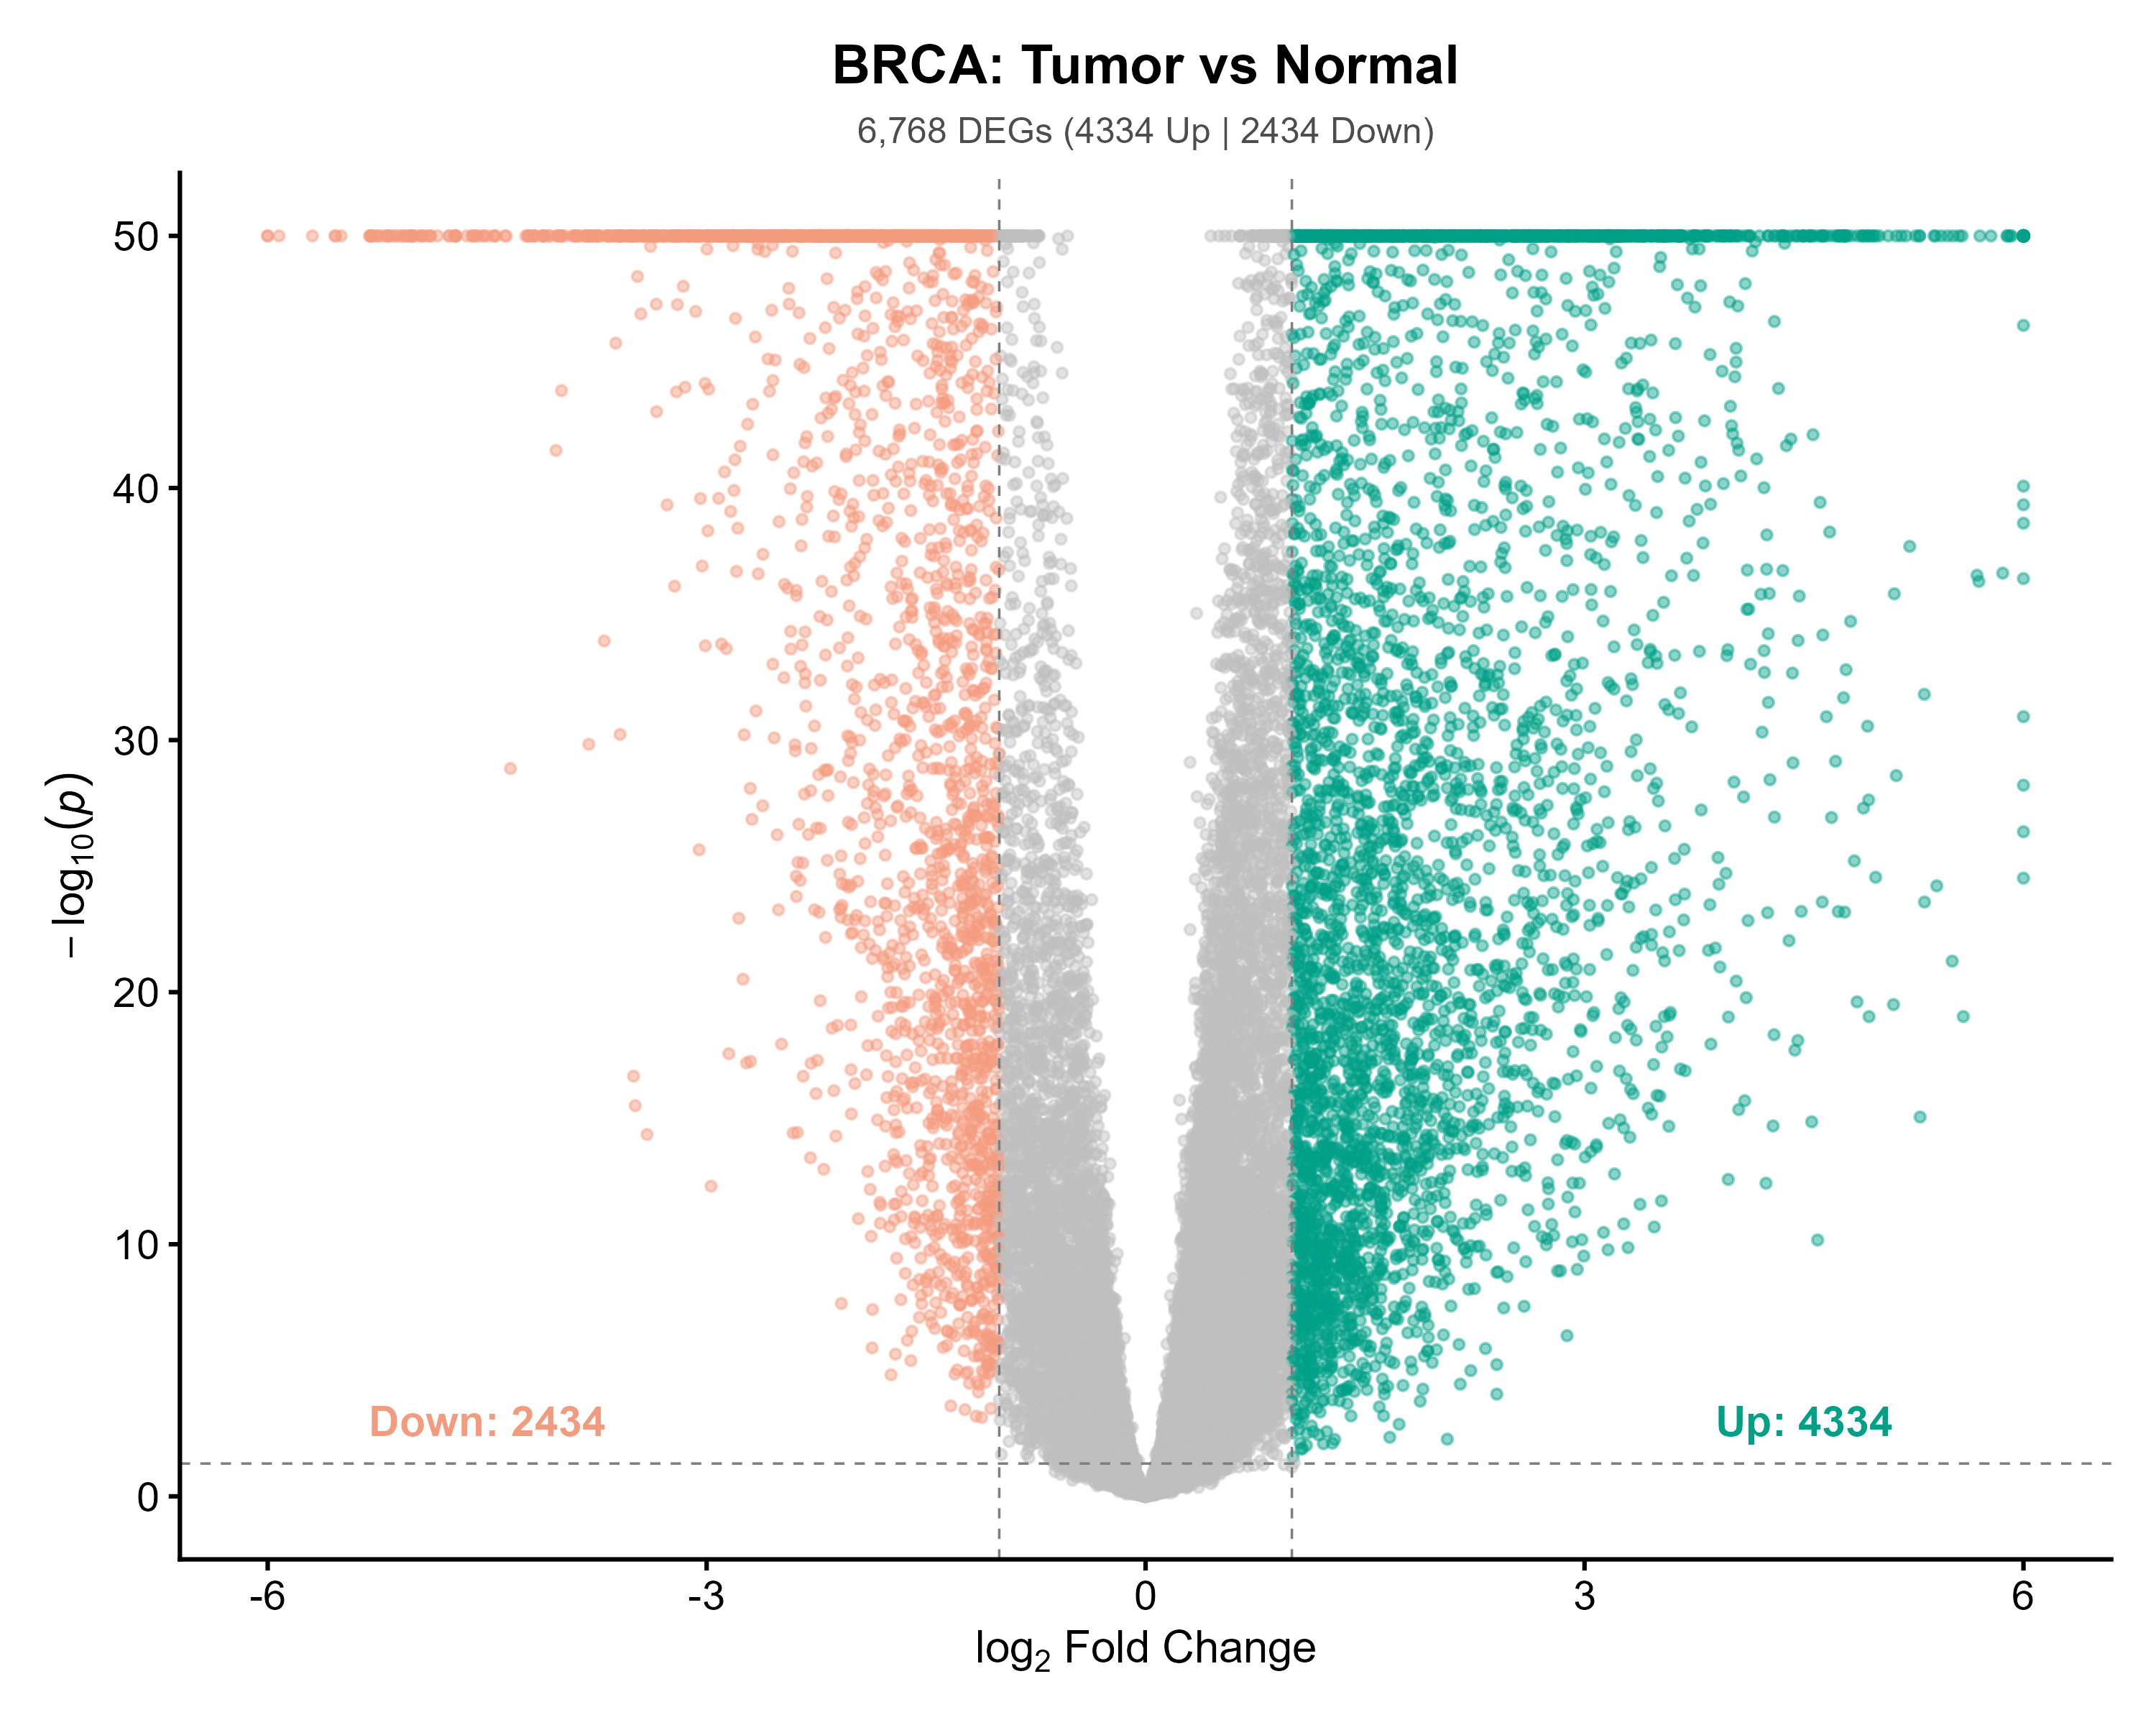
\includegraphics[width=0.85\textwidth]{fig1_volcano.png}
\caption{差异表达火山图（Tumor vs Normal）。横轴$\log_2$FC（$\pm6$），纵轴$-\log_{10}(p)$（50）。虚线上方且虚线外侧的点为满足$|\log_2\text{FC}|>1$且FDR$<0.05$的显著差异表达基因（6,768个）。NPG色板标注上调与下调方向：上调npg10[3]，下调npg10[5]，非显著grey75。ggrepel标注了显著基因的Gene Symbol。}\label{fig:volcano}
\end{figure}

\begin{table}[H]
\centering\caption{差异表达分析结果}\label{tab:deg}
\begin{tabular}{ll}\toprule
指标 & 数值 \\\midrule
总DEGs（$|\log_2\text{FC}|>1$, FDR$<0.05$） & 6,768 \\
上调基因数 & 4,334 \\
下调基因数 & 2,434 \\
分析方法 & DESeq2 (Wald test, BH correction) \\\bottomrule
\end{tabular}
\end{table}

\subsection{亚型间差异表达}
Triple Negative（$n=115$）与Luminal A（$n=950$）之间的差异表达分析鉴定出4,888个显著基因（$|\log_2\text{FC}|>1$, FDR$<0.05$），其中TN上调2,270个，Luminal A上调2,618个（图\ref{fig:tnla}）。与Tumor vs Normal火山图相比，TN vs Luminal A的差异分布呈现更加"大致均衡但LA偏多"的特征，说明乳腺癌不同分子亚型之间的差异并非单方向的转录激活，而更接近于两种不同转录程序之间的竞争性重塑。TN上调的数量（2,270）虽略少于LA（2,618），但考虑到TN仅115例而LA有950例，TN能在样本量悬殊的情况下驱动接近数量的上调基因，反映出TNBC内部更高的转录组异质性——这是TNBC已知的生物学特征。需要注意的是DEG数量受样本方差、离散度和异质性等多种因素共同影响，不能简单等同于"转录活性更强"。

\begin{figure}[H]
\centering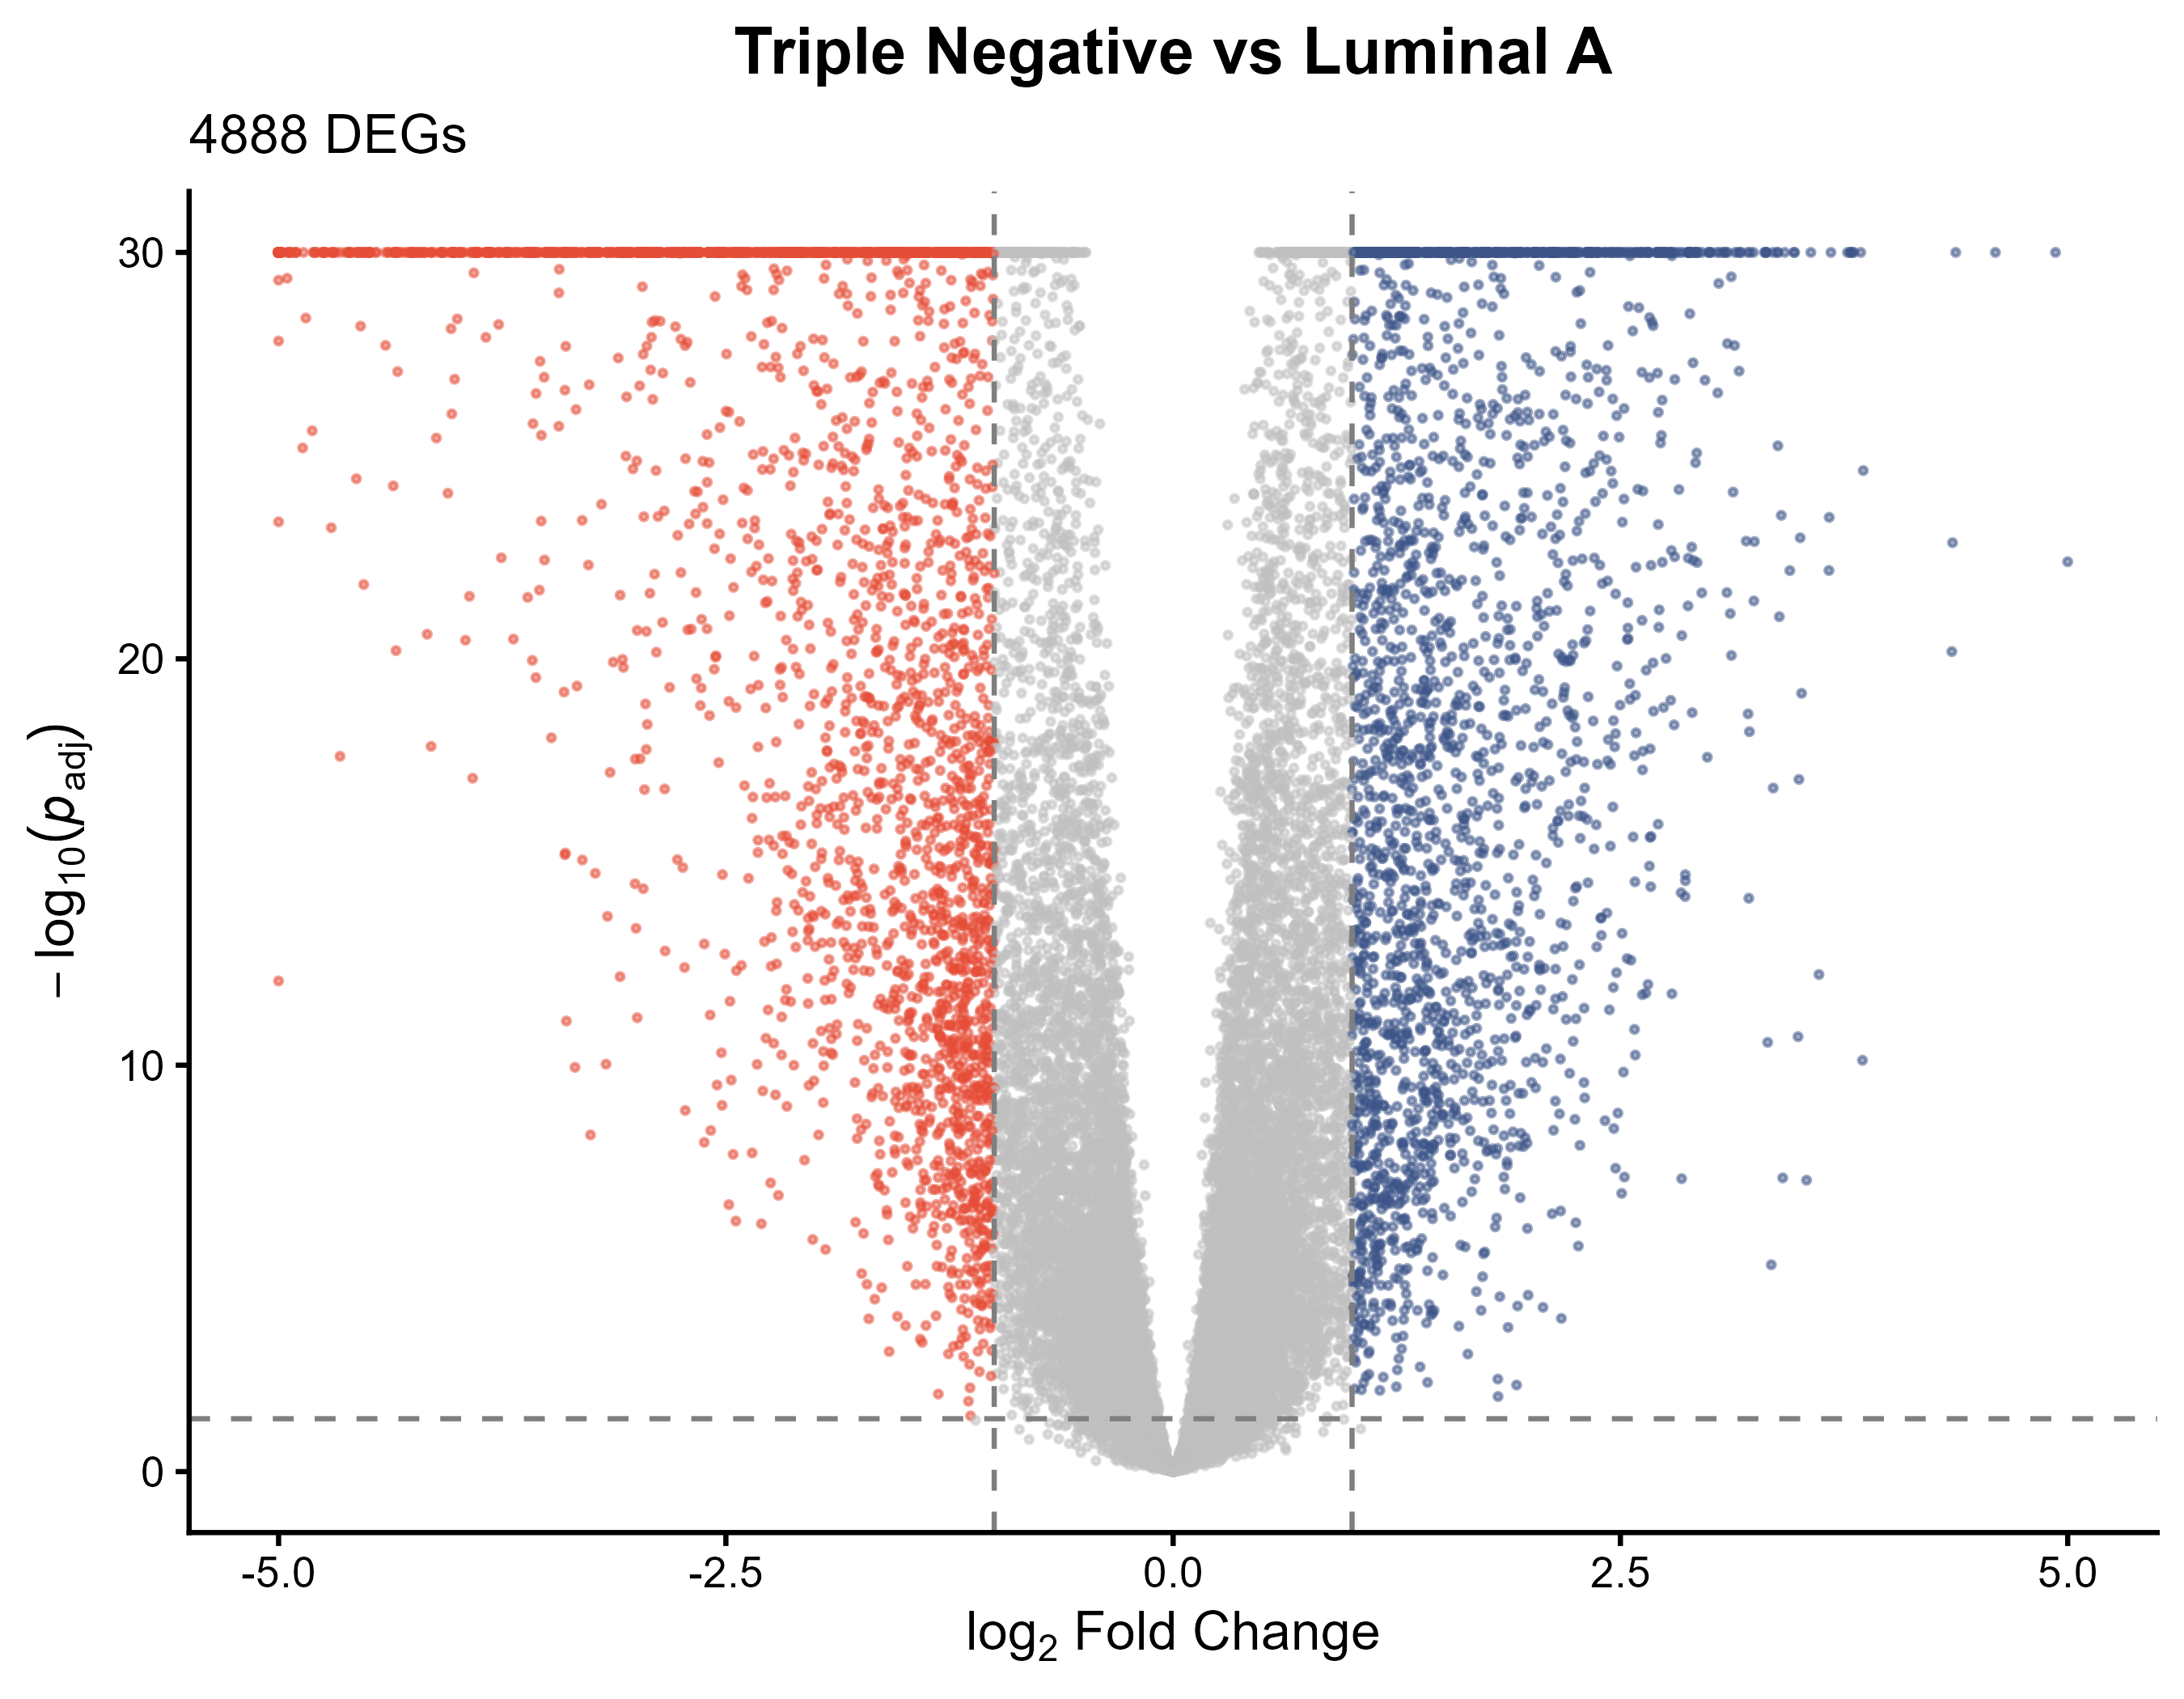
\includegraphics[width=0.85\textwidth]{fig17_tn_vs_la_volcano.png}
\caption{TN vs Luminal A差异表达火山图。横轴$\log_2$FC（$\pm5$），纵轴$-\log_{10}(p_{\text{adj}})$（30）。TN中上调npg10[4]（2,270个），Luminal A中上调npg10[1]（2,618个），非显著grey75。}\label{fig:tnla}
\end{figure}

\subsection{功能富集分析}
上调基因的富集信号呈现高度集中的特征（图\ref{fig:enrich_up}）。在643条显著条目（FDR$<0.05$）中，前五位全部来自Reactome数据库且集中于同一功能轴线：Cell Cycle（187个基因，$p=1.5\times10^{-21}$）居首，其后为Cell Cycle Mitotic（$p=3.7\times10^{-21}$）、Nucleosome assembly（$p=7.1\times10^{-21}$）以及Cell Cycle Checkpoints（$p=1.3\times10^{-18}$）。这些通路并非独立的生物学过程：Cell Cycle Mitotic和Cell Cycle Checkpoints是Cell Cycle层级下的子通路，Nucleosome assembly是DNA复制包装的必要步骤——它们共同构成细胞增殖轴线的多角度证据。六个来源数据库的条目分布为GO:BP 303条、Reactome 191条、GO:CC 75条、GO:MF 37条、WikiPathway 21条、KEGG 16条，GO:BP在条目数量上占优，但Reactome贡献了最强的显著性信号。Cell Cycle包含的187个交叠基因规模说明差异表达并非由少数关键基因驱动，而是整个细胞周期调控网络发生了系统性激活——这一结果与Hanahan\cite{hanahan2011hallmarks}提出的"持续增殖信号"特征高度吻合。

下调基因的富集方向截然不同（图\ref{fig:enrich_down}）。1,414条显著条目分布更为广泛，主要涉及细胞外基质组织（ECM organization）、细胞黏附（Cell adhesion）、脂质代谢及PI3K-Akt信号通路。下调条目总数远超上调（1,414 vs 643），暗示被抑制的生物学功能类别比被激活的更为分散。ECM organization和Cell adhesion的显著下调具有直接肿瘤生物学意义：细胞外基质和黏附系统是维持组织完整性的核心结构，其功能减弱意味着癌细胞更容易脱离原发位置并获得迁移和侵袭能力——这与肿瘤转移的经典机制一致。表\ref{tab:enrich}汇总了三组基因集的富集统计。

\begin{figure}[H]
\centering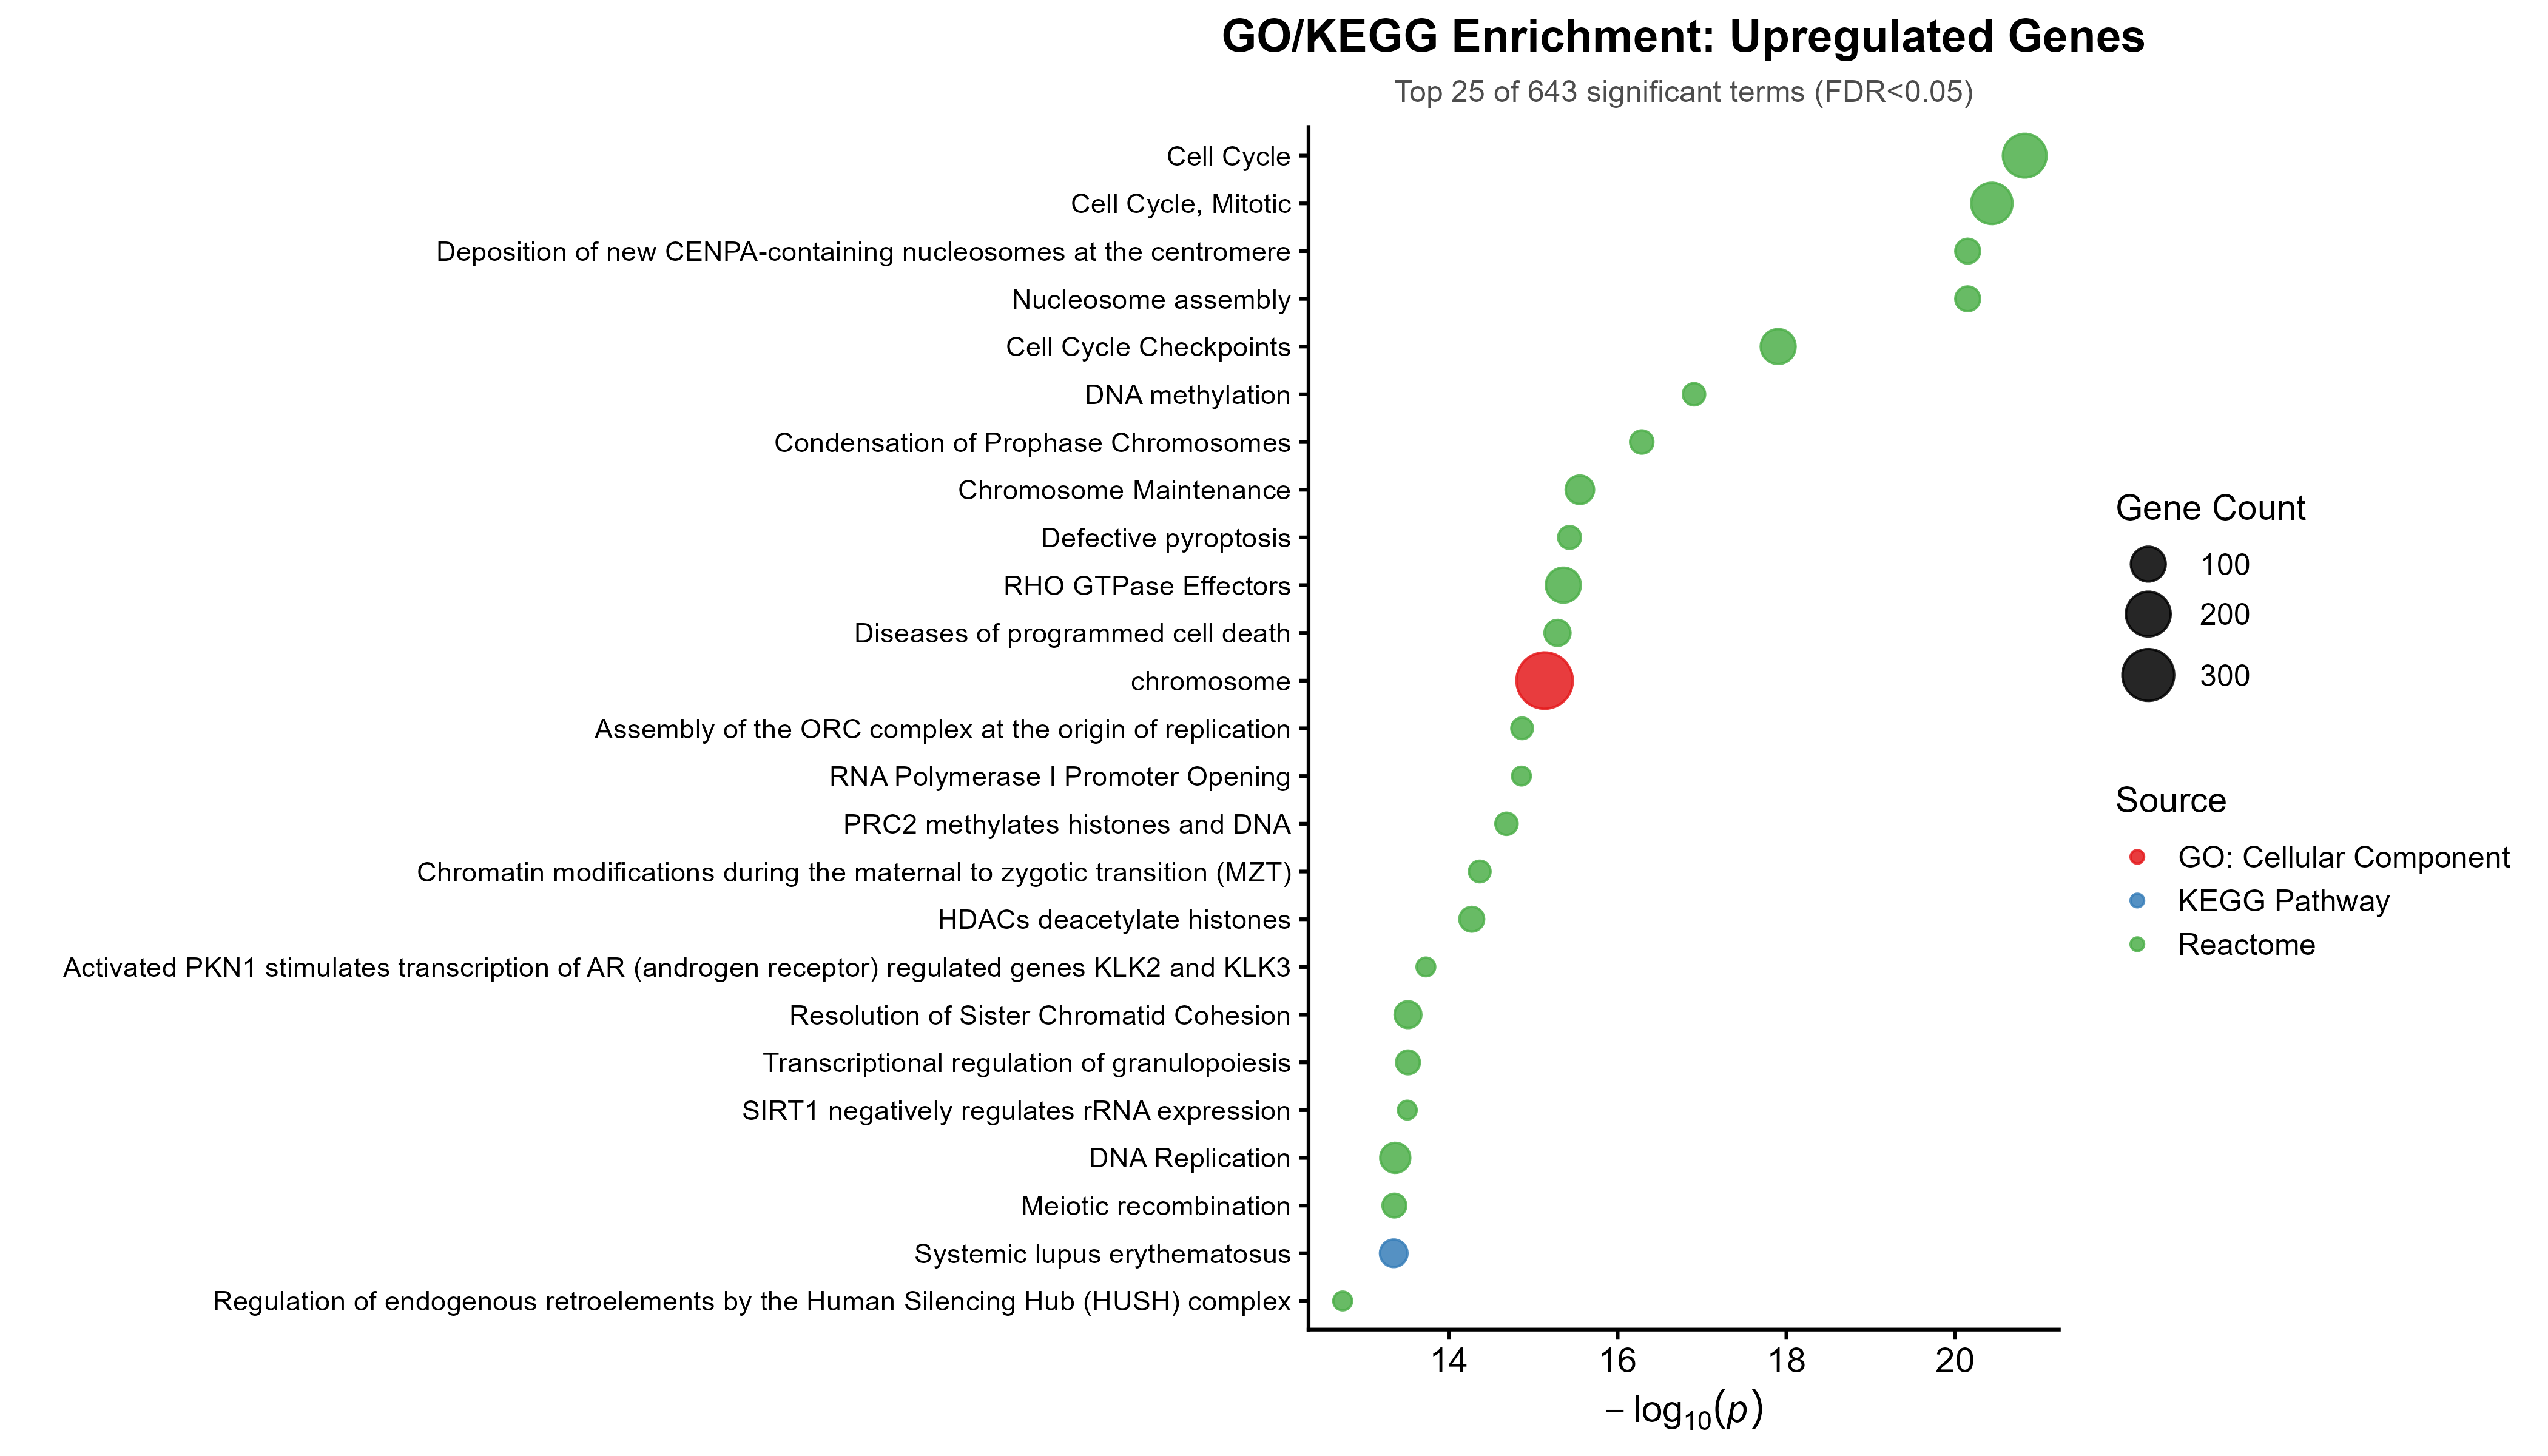
\includegraphics[width=0.85\textwidth]{fig12_enrichment_up.png}
\caption{上调基因富集气泡图（Top 25, FDR$<0.05$）。横轴$-\log_{10}(p)$，纵轴通路名称按显著性降序。气泡大小=交叠基因数量，颜色区分来源数据库（scale\_color\_brewer(palette="Set1")，六数据库）。前五位全部为Reactome细胞周期相关条目。}\label{fig:enrich_up}
\end{figure}

\begin{figure}[H]
\centering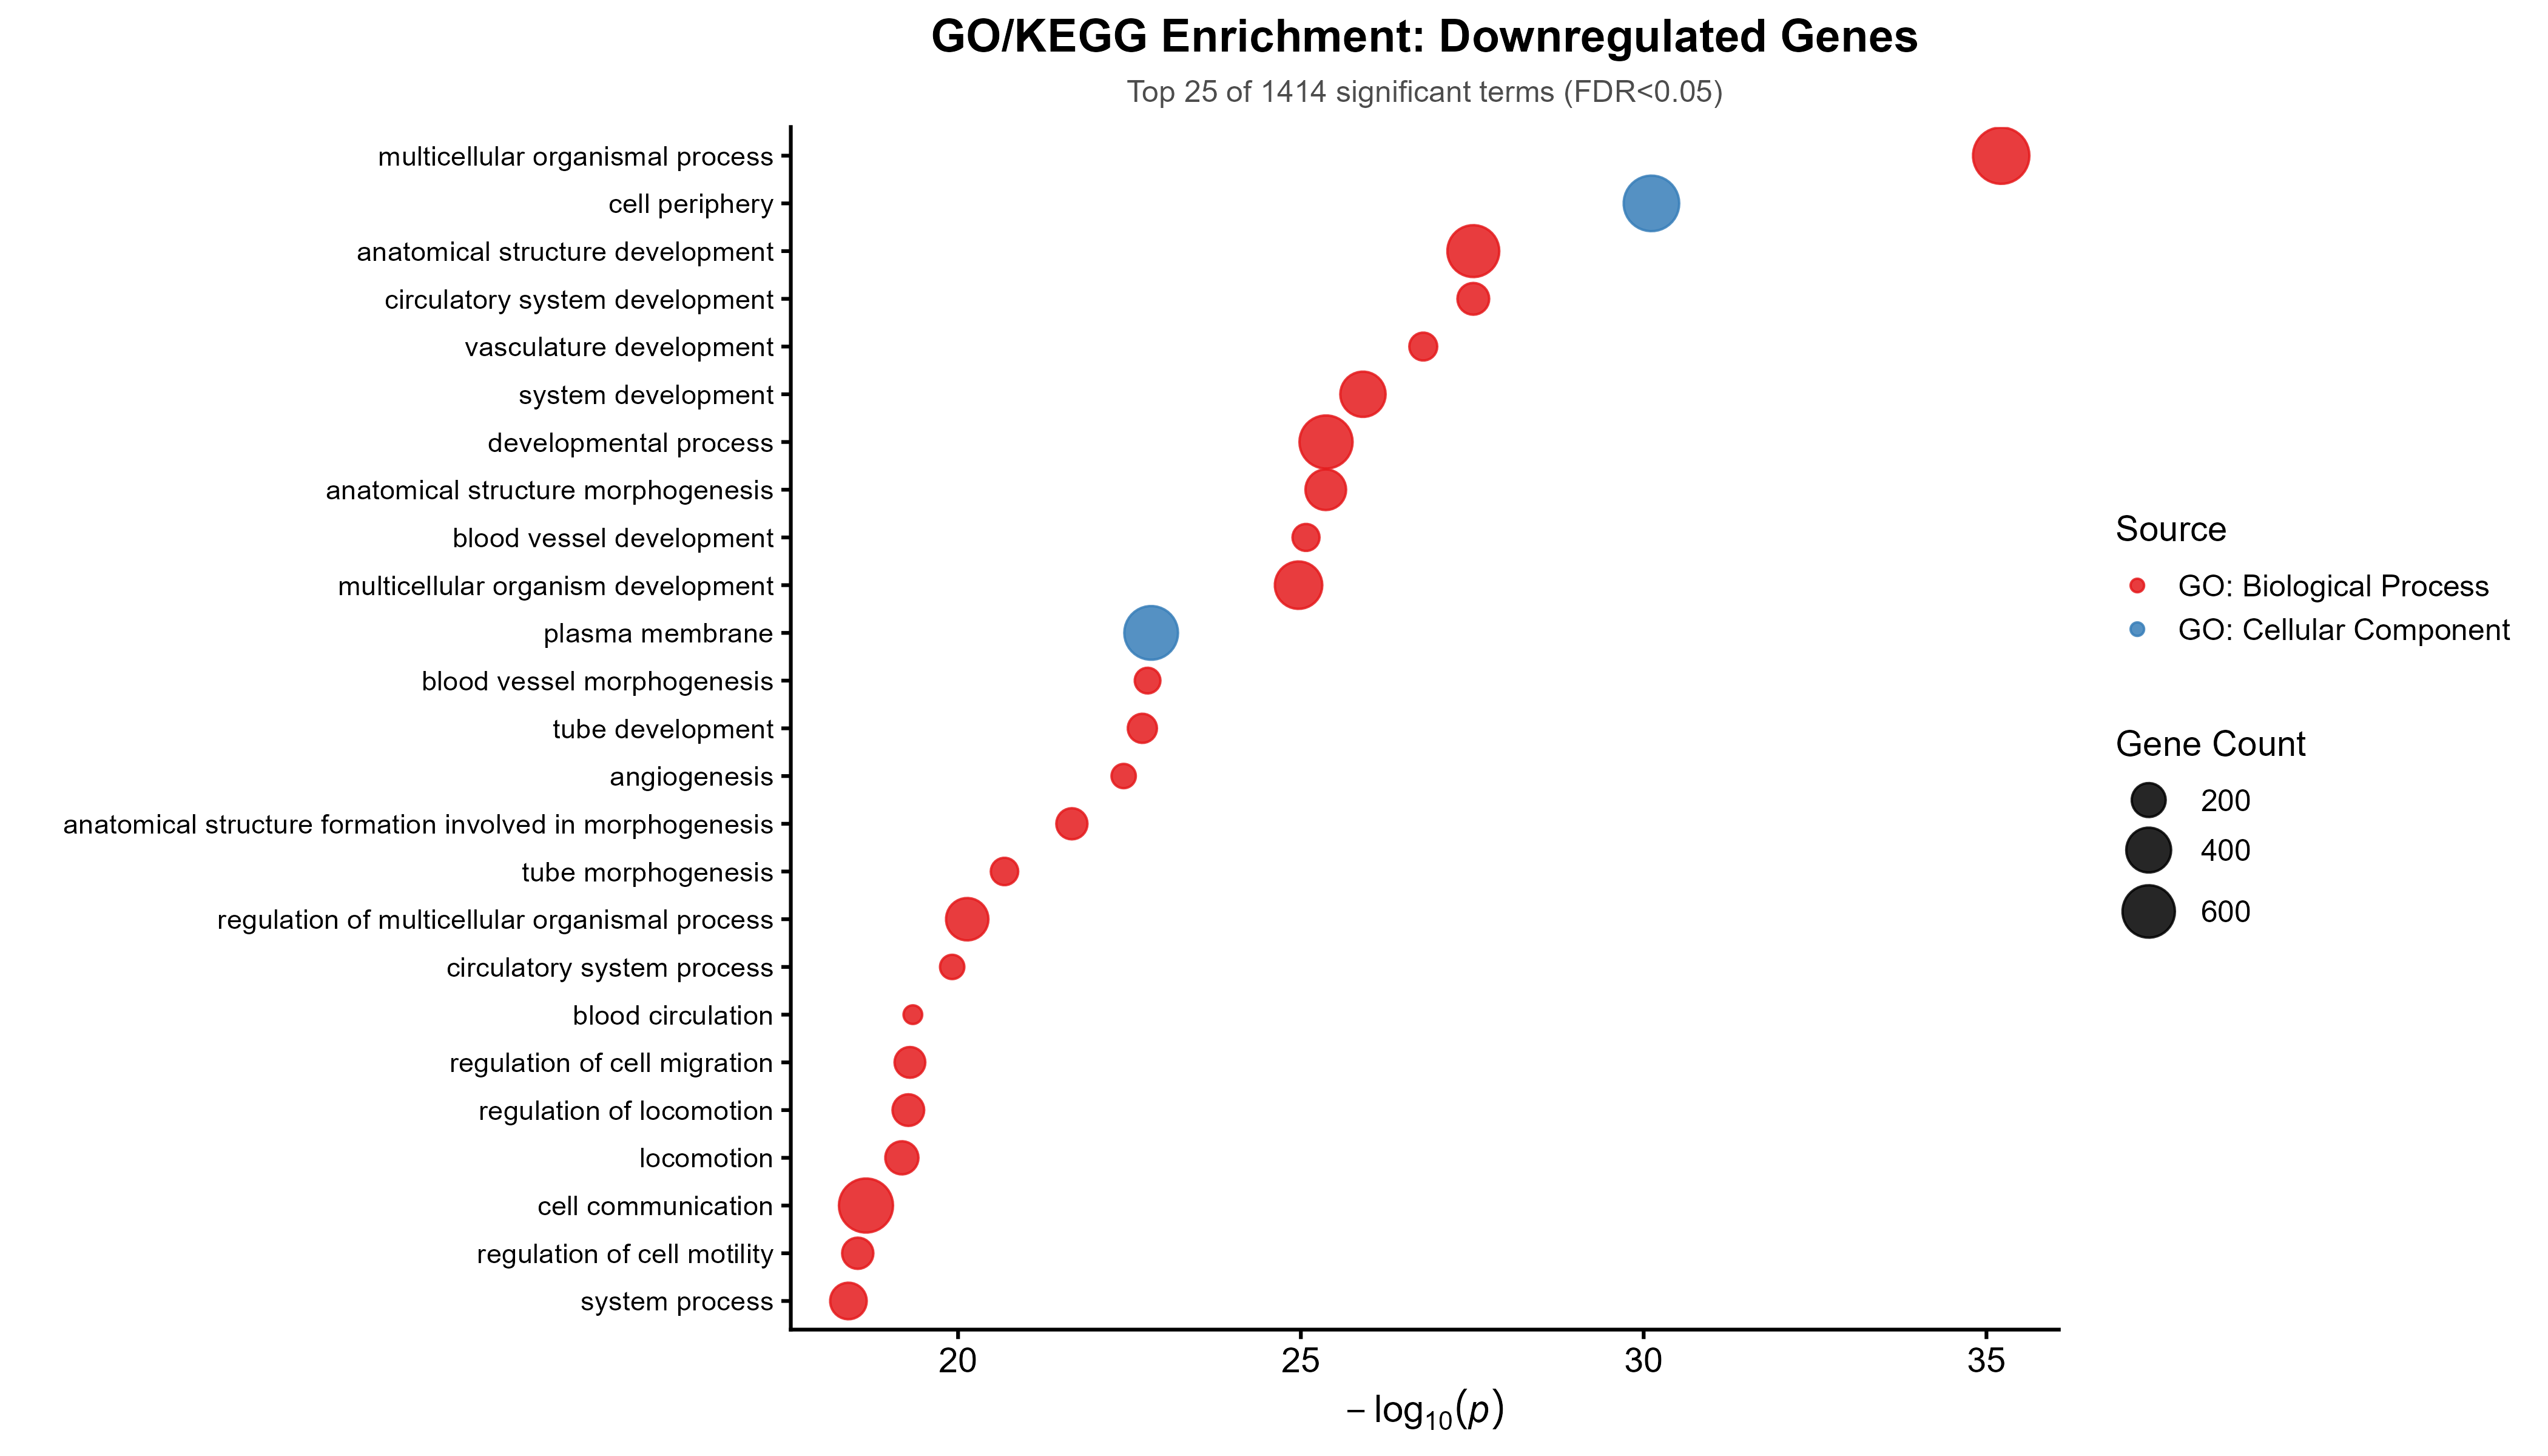
\includegraphics[width=0.85\textwidth]{fig13_enrichment_down.png}
\caption{下调基因富集气泡图（Top 25, FDR$<0.05$）。参数同上调图。分布较上调基因广泛，涉及ECM organization、Cell adhesion等多个功能方向。下调条目总数（1,414）超过上调（643）的两倍。}\label{fig:enrich_down}
\end{figure}

\begin{table}[H]
\centering\caption{功能富集分析结果汇总}\label{tab:enrich}
\begin{tabular}{lllll}\toprule
基因集 & 基因数 & 显著条目 & Top通路 & $p$值 \\\midrule
上调 & 4,334 & 643 & Cell Cycle (Reactome) & $1.5\times10^{-21}$ \\
下调 & 2,434 & 1,414 & ECM Organization (Reactome) & $\sim10^{-15}$ \\
全部DEGs & 6,768 & 1,280 & Cell Cycle (Reactome) & $\sim10^{-18}$ \\\bottomrule
\end{tabular}
\end{table}

\section{分子亚型分类}
三种分类器在独立测试集上的性能差异显著（图\ref{fig:model}，表\ref{tab:class}）。LASSO以89.4\%准确率排序第一（Kappa=0.528），仅使用从500个候选基因中筛选出的35个区分性基因——压缩比约为14:1。这一高压缩比揭示了BRCA分子亚型之间存在较强的稀疏判别结构：真正决定亚型分类的关键表达特征并不需要大量基因，而集中于少数具有高度判别能力的核心标志物。随机森林准确率为86.7\%（Kappa=0.365），其Macro F1分数（0.706）高于LASSO（0.612），这是因为F1 Macro对每个类别等权重计算，随机森林在少数类（HER2-enriched仅37例、Triple Negative仅115例）上保持了更好的召回率。在类别不平衡的医学分类任务中，单纯追求Accuracy往往容易偏向多数类，而Macro F1更能反映模型对所有亚型的综合识别能力。

XGBoost的准确率仅为35.8\%（Kappa=0.002），几乎等同于三分类随机猜测水平（33.3\%）。失败的可能原因包括默认超参数未针对该高维小样本数据集（772例训练、500个特征）进行调优，以及类别不平衡（三类的样本量为950/37/115）可能加剧了模型的训练困难。此外，不排除存在标签编码或objective参数设置的潜在问题——后续需通过网格搜索和交叉验证进行系统排查。这一结果说明复杂模型并不一定适用于高维小样本组学数据——在样本量有限的条件下，过于灵活的非线性模型更容易出现参数不稳定和过拟合，而LASSO这类具有强正则化约束的方法反而表现更优。更深层地看，对于BRCA转录组分类问题，"特征质量"比"模型复杂度"更加重要。

\begin{figure}[H]
\centering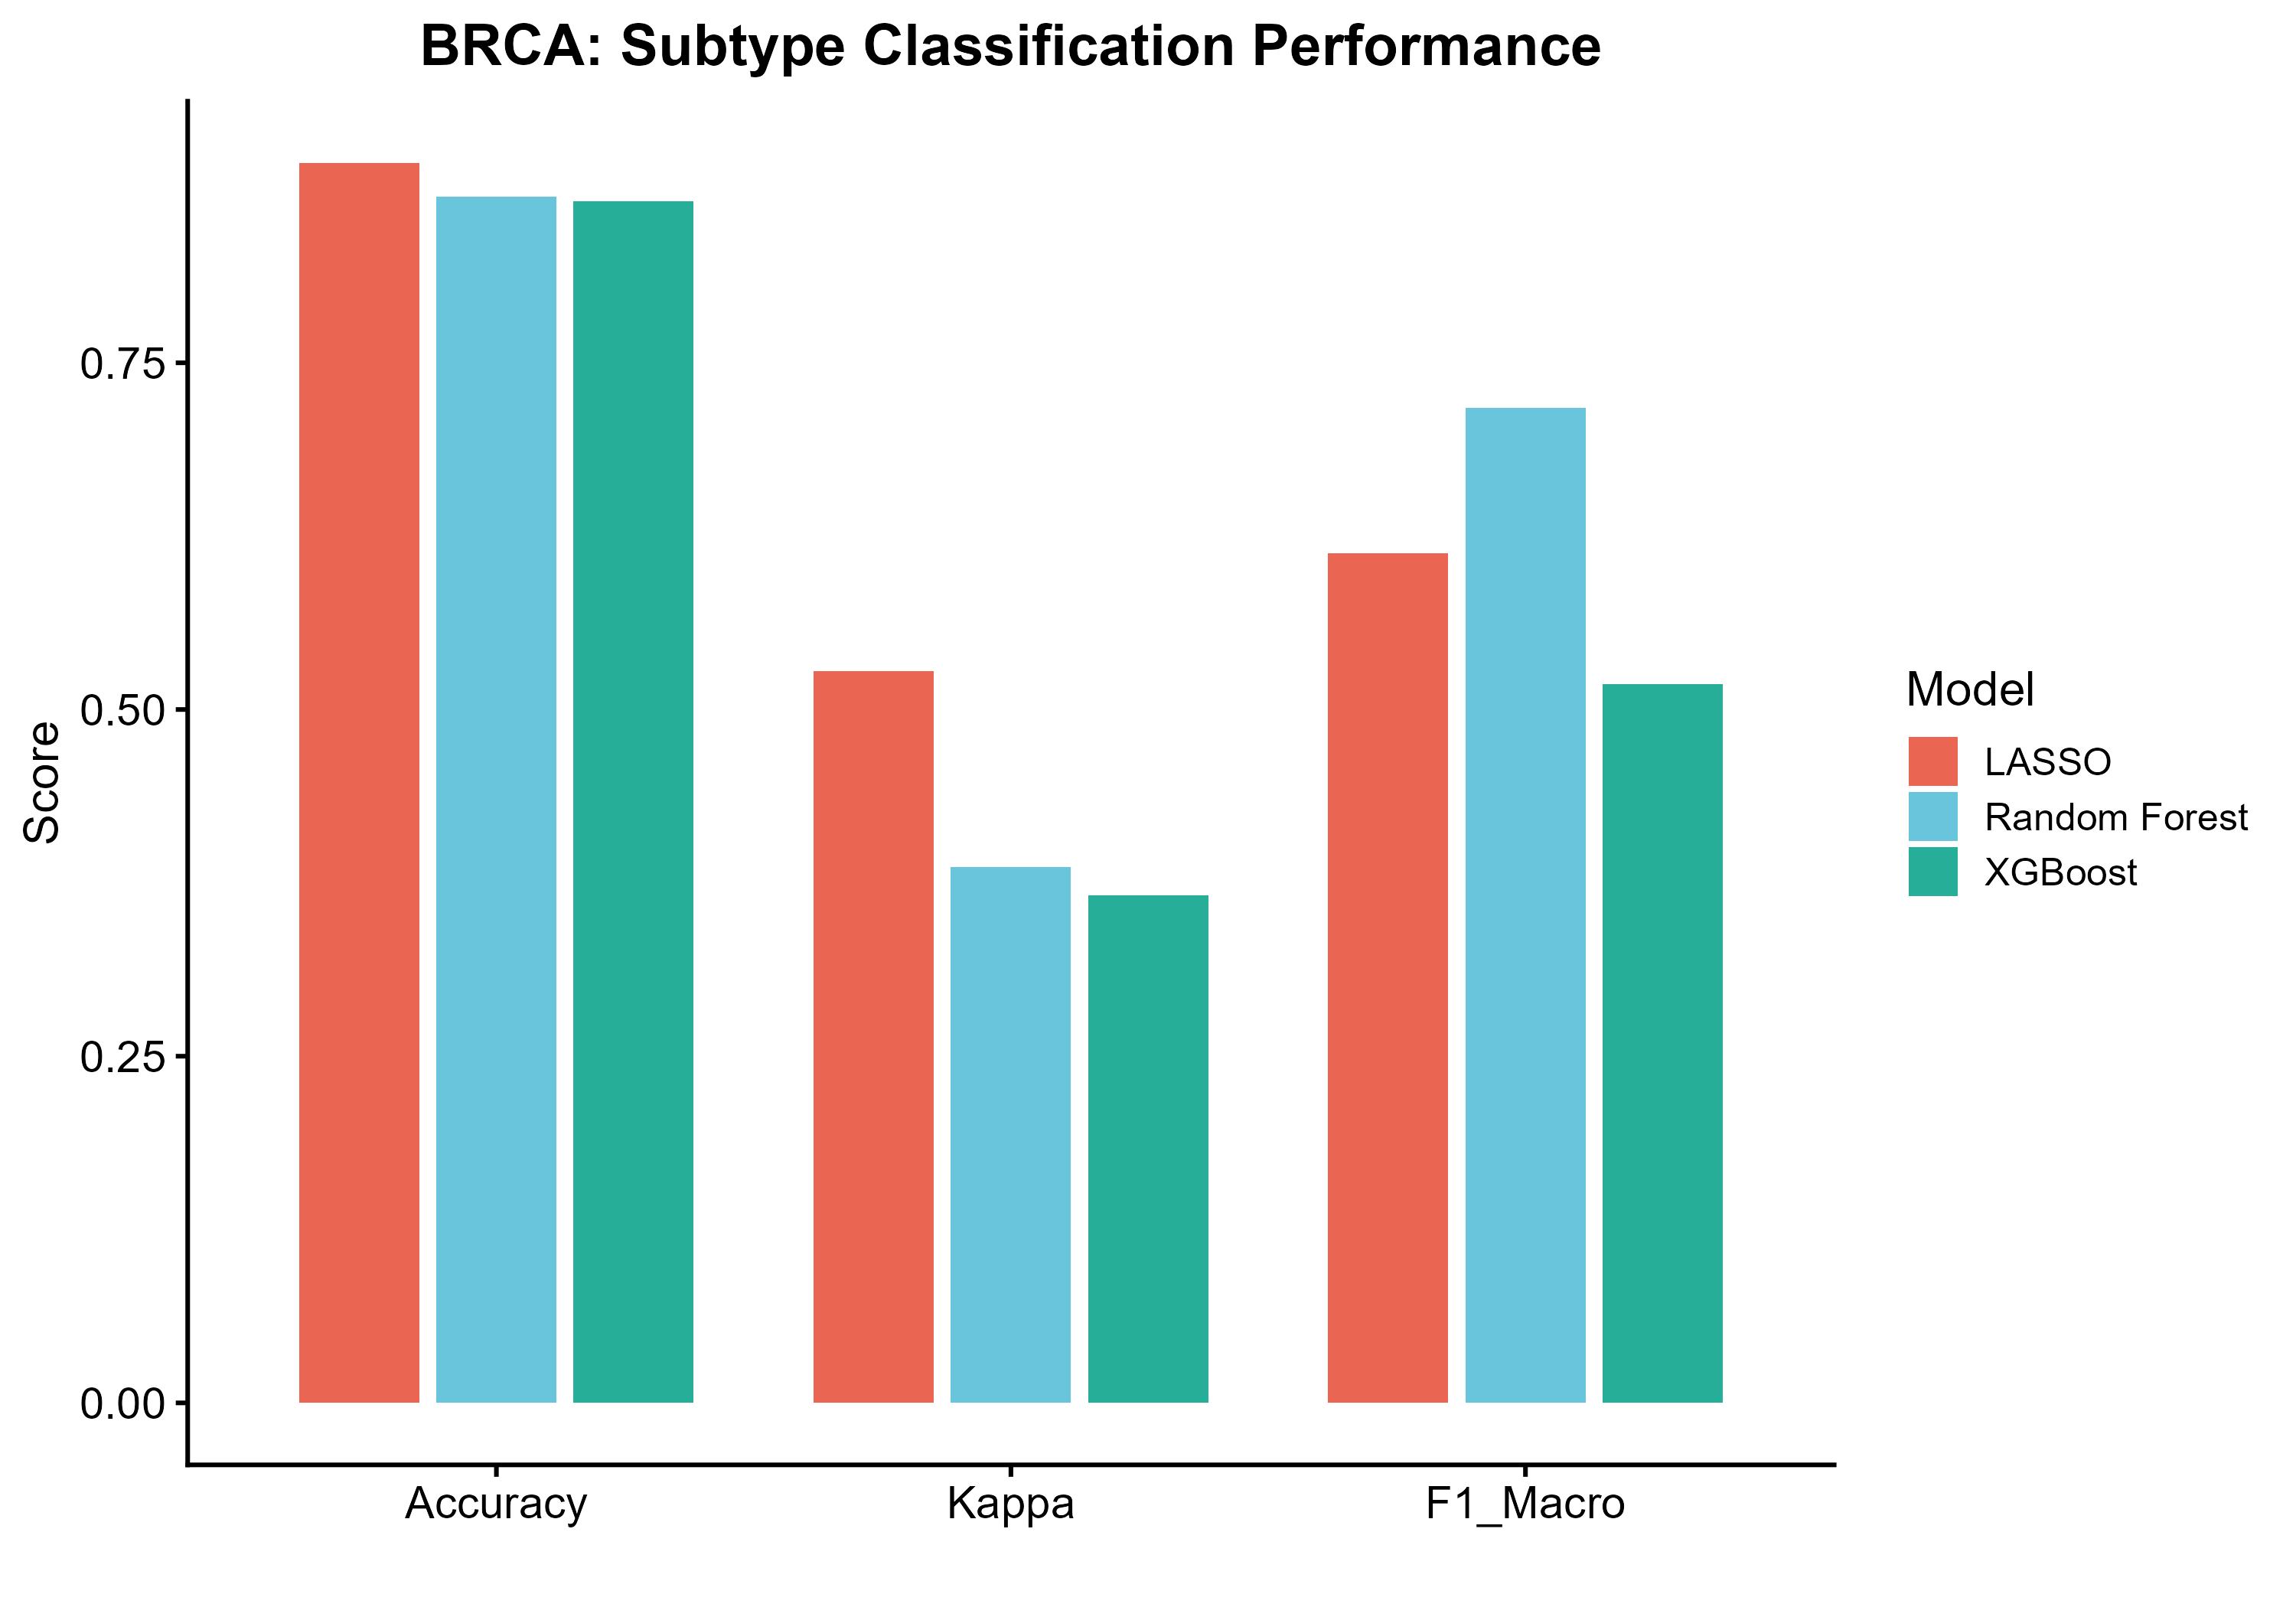
\includegraphics[width=0.7\textwidth]{fig6_model_comparison.png}
\caption{分类模型性能对比分组柱状图。每组三根柱分别对应Accuracy、Kappa和F1 Macro。绘图参数：fill=npg10[1:3]（3种模型）。LASSO在Accuracy和Kappa上最优，RF在F1 Macro上最优。}\label{fig:model}
\end{figure}

\begin{table}[H]
\centering\caption{分子亚型分类模型性能对比}\label{tab:class}
\begin{tabular}{lllll}\toprule
模型 & Accuracy & Kappa & F1 (Macro) & 特征数 \\\midrule
LASSO (Multinomial) & 0.894 & 0.528 & 0.612 & 35 \\
Random Forest & 0.867 & 0.365 & 0.706 & 500 \\
XGBoost & 0.358 & 0.002 & 0.232 & 500 \\\bottomrule
\end{tabular}
\end{table}

\section{聚类分析}
PCA分析结果（图\ref{fig:pca}）展示了BRCA转录组的宏观连续谱结构。PC1解释了15.3\%的总方差，PC2解释了8.5\%，合计23.8\%。虽然解释率并非极高，但这已足以在二维空间中形成明显的亚型分离趋势。沿PC1方向，Luminal A样本紧密聚集于负值区域——其95\%置信椭圆面积明显较小，提示该亚型内部具有较高的一致性，这与临床上Luminal A生物学行为较稳定、预后较好的特点一致。Triple Negative样本散布于正值区域且离散度明显更大，这种"扩散型"结构意味着TNBC内部存在更强的转录组异质性——虽然TNBC在临床上被归为同一类别，但其内部可能仍包含多个潜在分子子群。HER2-enriched样本居中，提示其可能在部分分子特征上兼具ER+和ER-两种亚型的属性，进一步说明乳腺癌亚型之间并不存在绝对边界，而更接近于连续的分子状态过渡。

PC1方向上的分离与ER状态显著相关。由于未进行主成分载荷分析和ER通路特异性富集验证，此处仅能报告关联性而非因果驱动关系。K-means轮廓系数在$K=2$时达到最大值0.18，之后随$K$增大单调递减。最佳$K=2$与PCA的视觉图景一致——ER+/ER-是BRCA转录组数据中相对最显著的分组结构。然而，需指出silhouette系数最大值仅为0.18，说明数据中并不存在高度紧凑且边界清晰的聚类结构，进一步验证了肿瘤转录组的连续性本质。PC1解释率仅为15.3\%这一事实也提醒我们：即便当前分子分型体系已具有较高临床价值，BRCA内部仍可能存在尚未被充分定义的隐含分子结构——绝大多数转录组变异维度并不与已知分类标签对齐，这部分"未解释方差"是未来分型精细化的主要空间。

\begin{figure}[H]
\centering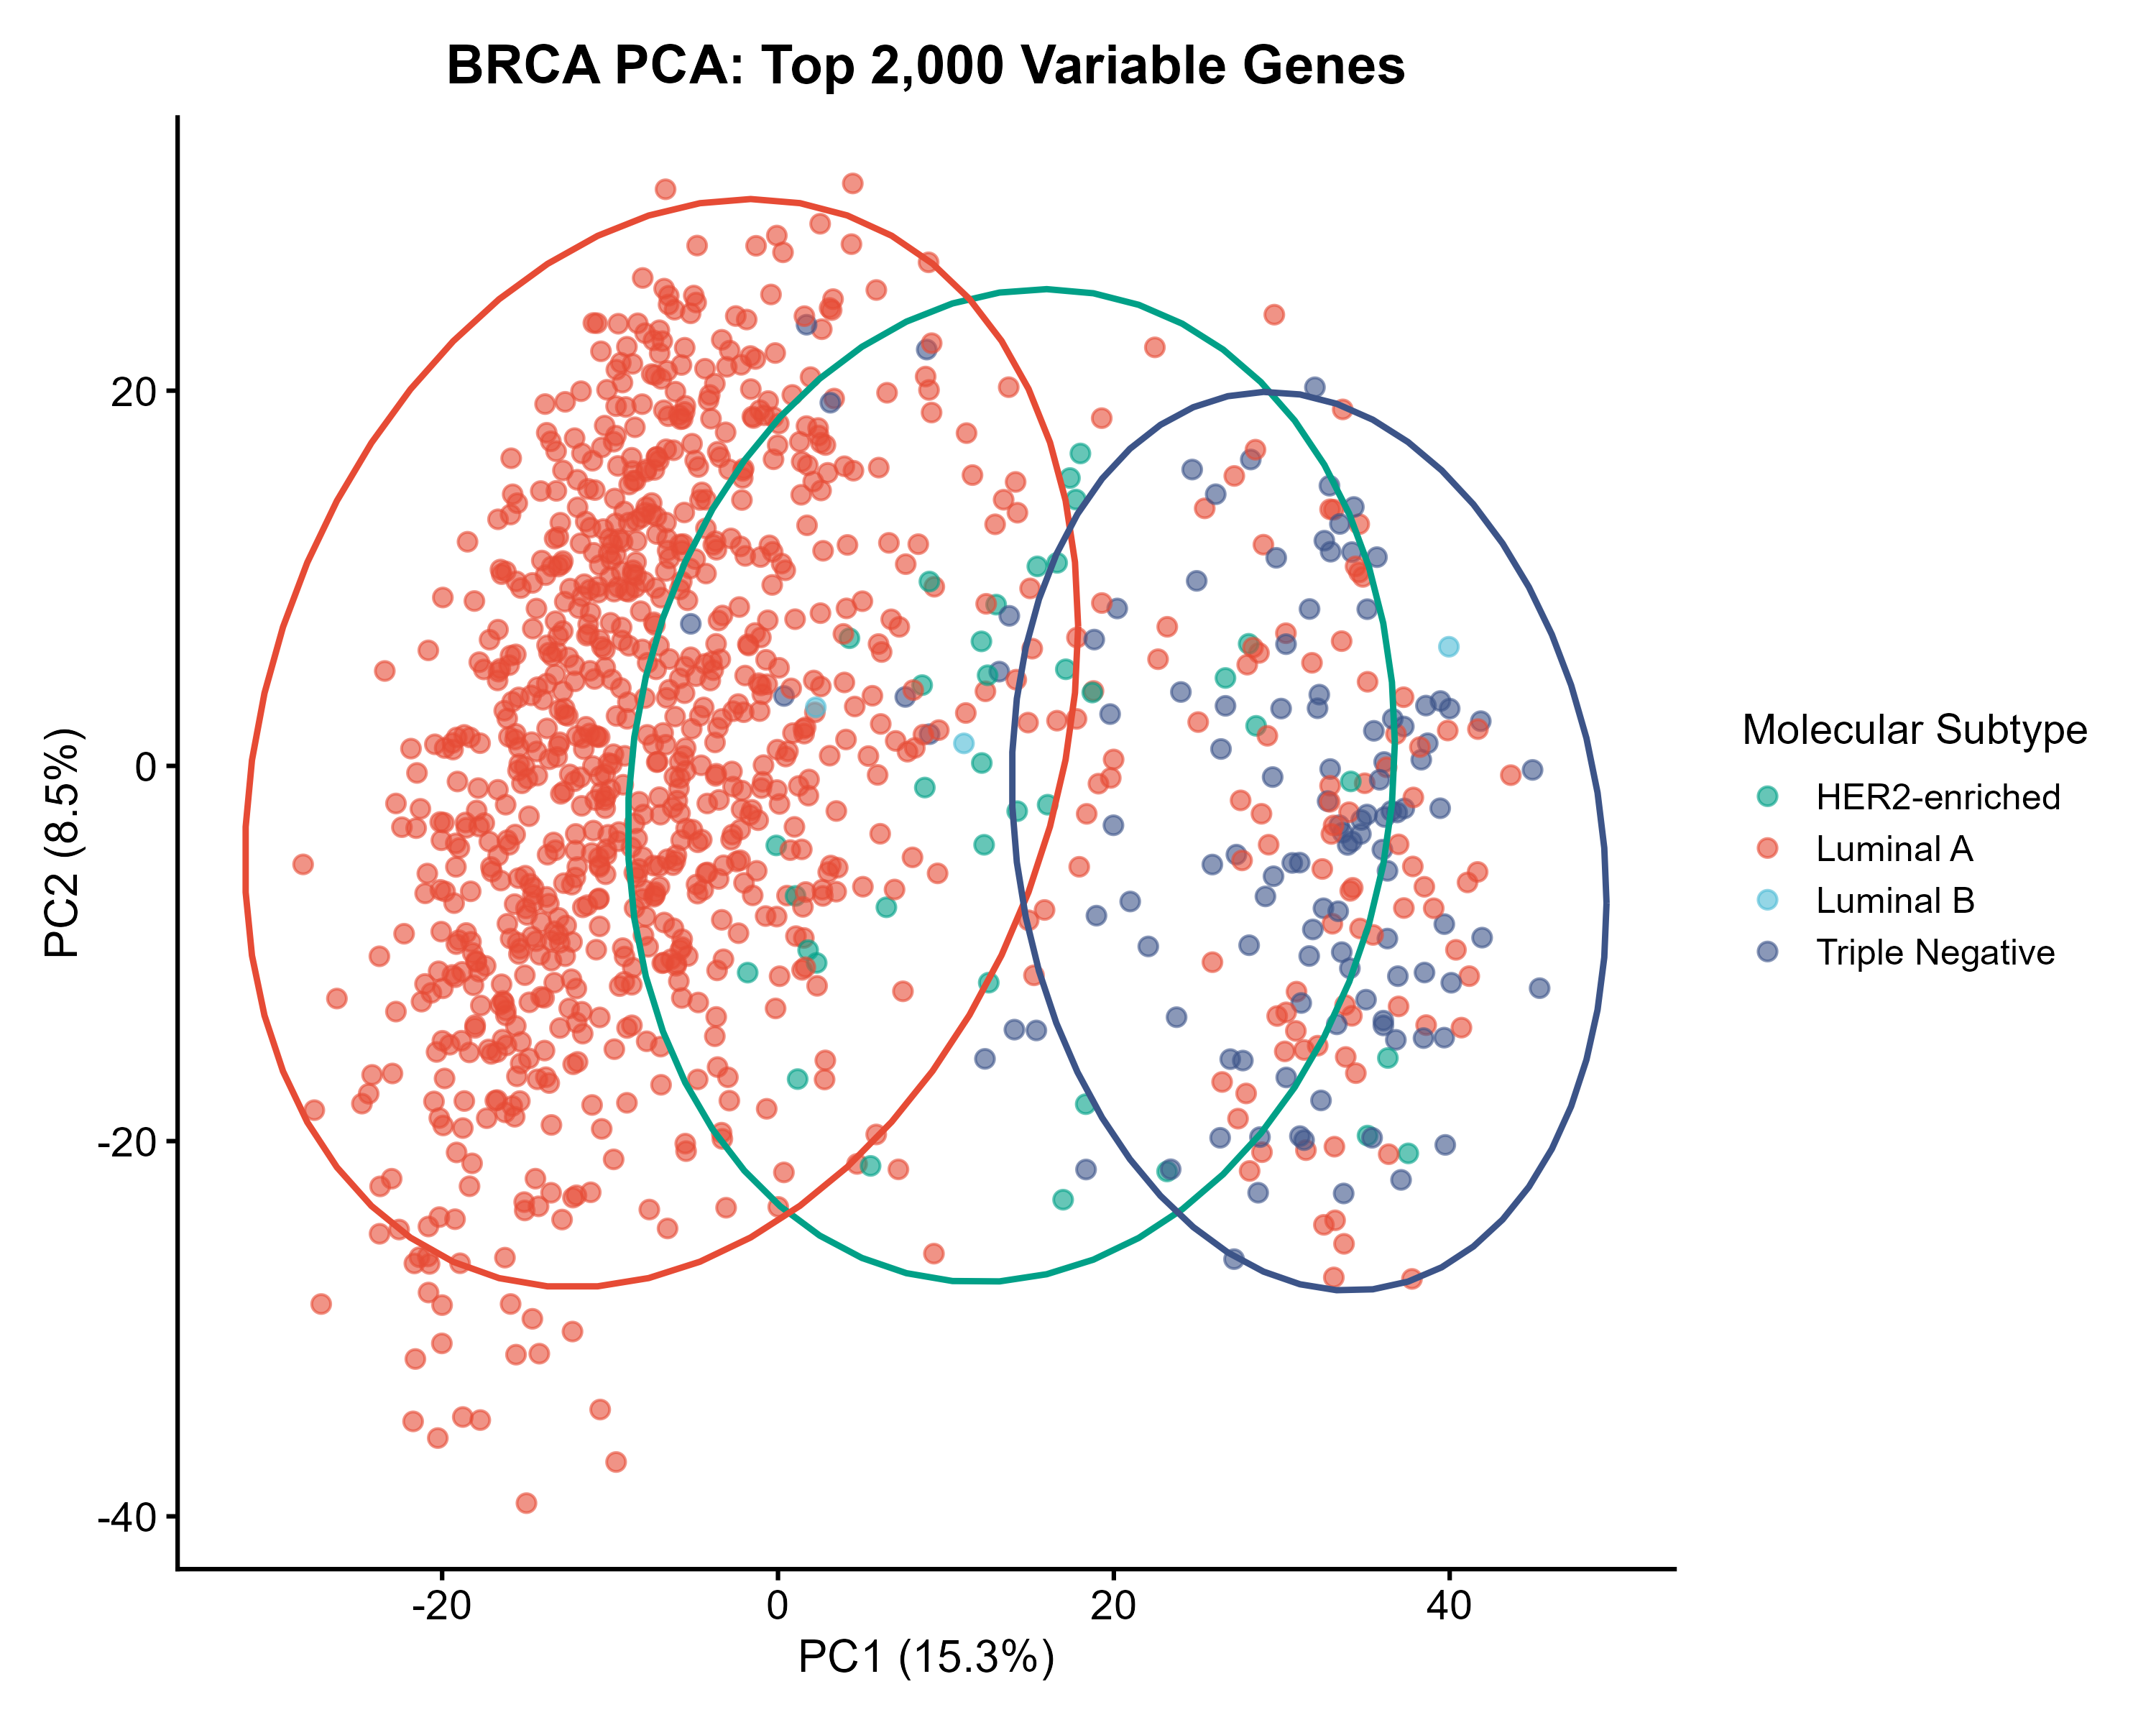
\includegraphics[width=0.85\textwidth]{fig2_pca_subtype.png}
\caption{PCA主成分分析（Top 2,000可变基因, 95\%置信椭圆）。绘图参数：Luminal A=npg10[1], Luminal B=npg10[2], HER2-enriched=npg10[3], Triple Negative=npg10[4]。注意Luminal B仅3例在图中几乎不可见——分类模型已将其过滤（仅使用3类）。PC1方向按ER状态分离；LA簇最紧凑，TN离散度最大，HER2居中。}\label{fig:pca}
\end{figure}

\section{WGCNA共表达网络}
软阈值选择曲线（图\ref{fig:wgcna}）展示了WGCNA网络构建过程中无标度拓扑假设的建立过程。左面板中$R^2$随Power增加而提高，在Power=7时首次突破0.8阈值（0.817），在Power=8时达到0.887。这意味着网络结构已经较好地接近真实生物网络常见的无标度特征。右面板展示平均连接度随Power的衰减——若Power过高，虽然$R^2$会进一步提高，但大量弱连接会被过度削弱，导致网络信息丢失。因此Power=8实际上是在"网络真实性"和"信息保留"之间取得的平衡点——这不仅是参数选择过程的展示，也是WGCNA方法学合理性的可视化证明。

经动态树切割和合并后，共识别8个有效共表达模块，另含grey未分配基因集（表\ref{tab:wgcna}）。grey模块（2,817个基因）容纳了56.3\%的输入基因。8个有效模块中，turquoise（584基因）和blue（553基因）规模最大。blue模块枢纽基因的$|\text{MM}|=0.959$为所有模块最高，表明该基因在所属共表达网络中处于核心调控位置。

\begin{figure}[H]
\centering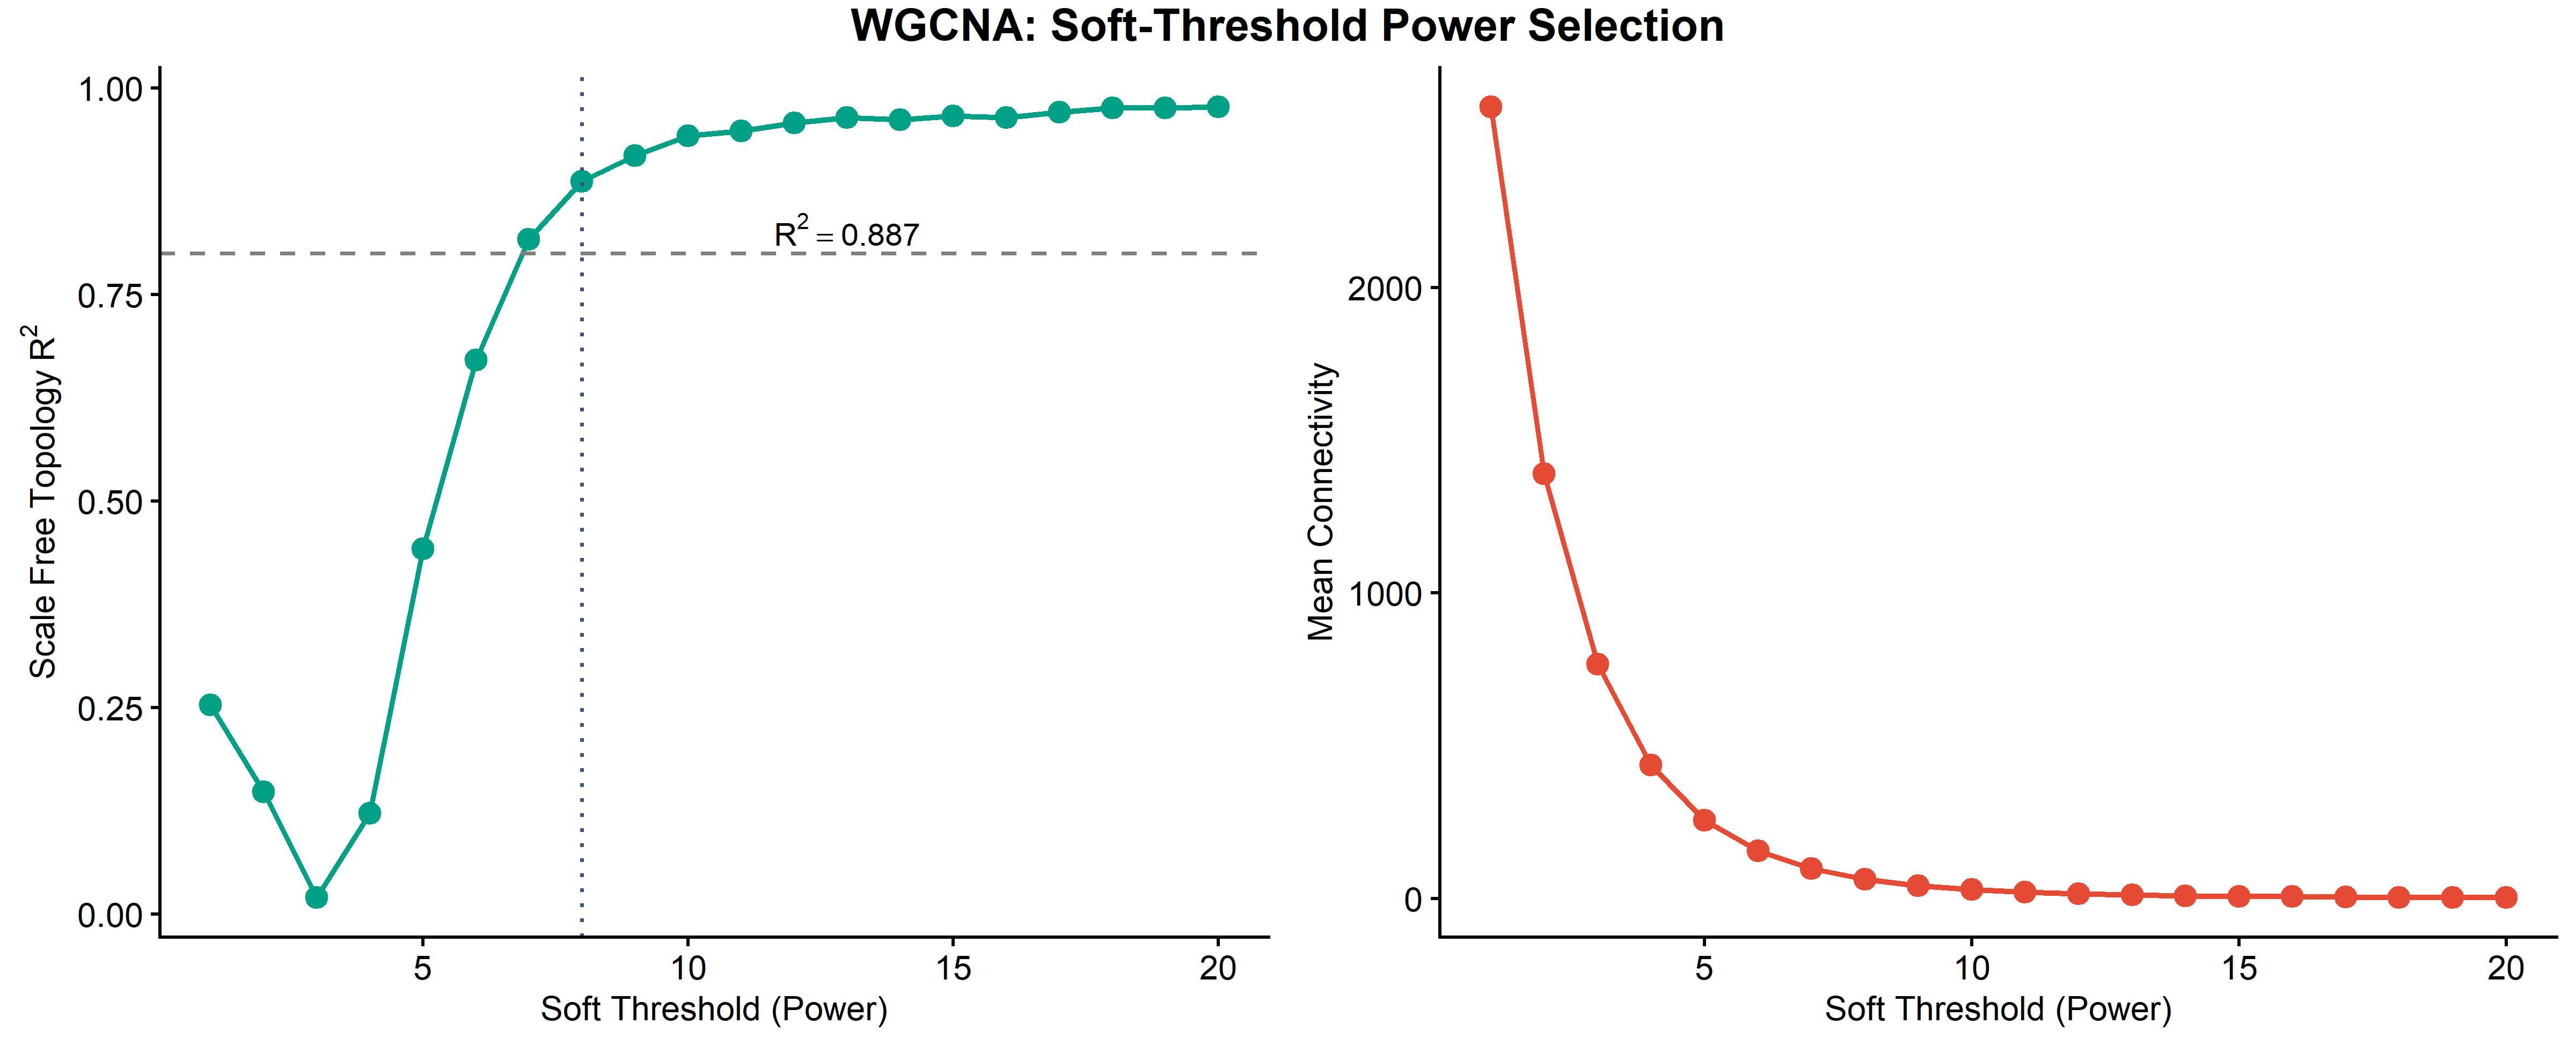
\includegraphics[width=0.95\textwidth]{fig7_wgcna_sft.png}
\caption{WGCNA软阈值选择。左：$R^2$ vs Power（虚线$R^2=0.8$, Power=8时$R^2=0.887$）。右：平均连接度 vs Power。绘图参数：SFT点/线=npg10[3], Mean Conn点/线=npg10[1]。}\label{fig:wgcna}
\end{figure}

\begin{table}[H]
\centering\caption{WGCNA共表达模块}\label{tab:wgcna}
\begin{tabular}{lll}\toprule
模块 & 基因数 & 枢纽基因$|\text{MM}|$ \\\midrule
grey（未分配，非有效模块） & 2,817 & — \\\\
turquoise & 584 & 0.889 \\
blue & 553 & 0.959 \\
brown & 336 & 0.911 \\
yellow & 260 & 0.874 \\
green & 224 & 0.903 \\
red & 119 & 0.881 \\
black & 63 & 0.854 \\
pink & 44 & 0.847 \\\\\midrule\multicolumn{3}{l}{\footnotesize *grey为未分配基因集合，不构成共表达模块，未计算枢纽基因} \\\\\bottomrule
\end{tabular}
\end{table}

\section{生存分析}
Kaplan-Meier曲线（图\ref{fig:km}）展示了按病理分期分层的总体生存情况。四条曲线自随访早期开始便逐渐拉开，并在整个观察周期内保持稳定间距，说明分期差异不仅影响短期死亡风险，也持续影响长期预后。Stage IV曲线下降最为陡峭——在5年时间点，其生存概率已降至约40\%以下，而Stage I的生存概率仍维持在约95\%，两组之间的绝对差异超过55个百分点。曲线之间几乎不存在明显交叉，意味着不同分期之间的风险排序在时间维度上保持稳定，符合Cox比例风险模型的基本假设。图下方的Number at Risk表标注了各随访节点的存活样本数——当随访后期剩余样本数显著减少时（如Stage IV的20例在5年时仅剩个位数），曲线尾部波动可能受到随机性影响，因此风险表对后期曲线稳定性的判断具有重要参考价值。log-rank检验$p<0.0001$表明分期间的生存差异远非随机波动所能解释。

Cox回归森林图（图\ref{fig:cox}）量化了各因素的独立预后贡献。横轴采用对数尺度以避免高风险变量在普通线性坐标中压缩其他变量的可视化空间。Stage IV的HR为30.36（95\%CI: 9.87--93.45, $p=2.67\times10^{-9}$），Stage III的HR为5.74（95\%CI: 2.09--15.79, $p=0.0007$），Stage II的HR为3.21（95\%CI: 1.27--8.12, $p=0.014$）。年龄也显示出显著的独立预后效应（HR=1.04/年, 95\%CI: 1.02--1.06, $p=8.19\times10^{-6}$）。Stage IV误差条相对较宽——因为IV期样本量仅20例，导致估计方差增大——但即便取CI的下限（9.87），晚期诊断仍意味着近10倍的死亡风险增加。Triple Negative在多变量模型中呈现边际显著（HR=2.00, 95\%CI: 1.08--3.71, $p=0.028$），在控制分期后仍对预后有一定独立贡献。HER2-enriched（HR=0.97, 95\%CI: 0.24--3.97）则不显著。模型整体C-index=0.771（似然比$p=8.62\times10^{-12}$）（表\ref{tab:cox}）。需要指出，Stage IV仅20例（其中死亡10例），在全部87个死亡事件中占比较小，因此其极高的HR（30.36）和超宽置信区间（9.87--93.45）部分反映了小样本条件下效应估计的不稳定性——这一结果的方向是明确的（晚期诊断显著增加死亡风险），但效应量幅度的精确解读需要更大队列的验证。此外，Cox比例风险假设未经过Schoenfeld残差检验的正式验证，仅通过KM曲线目视判断，这是本分析的一个方法学局限。

\begin{figure}[H]
\centering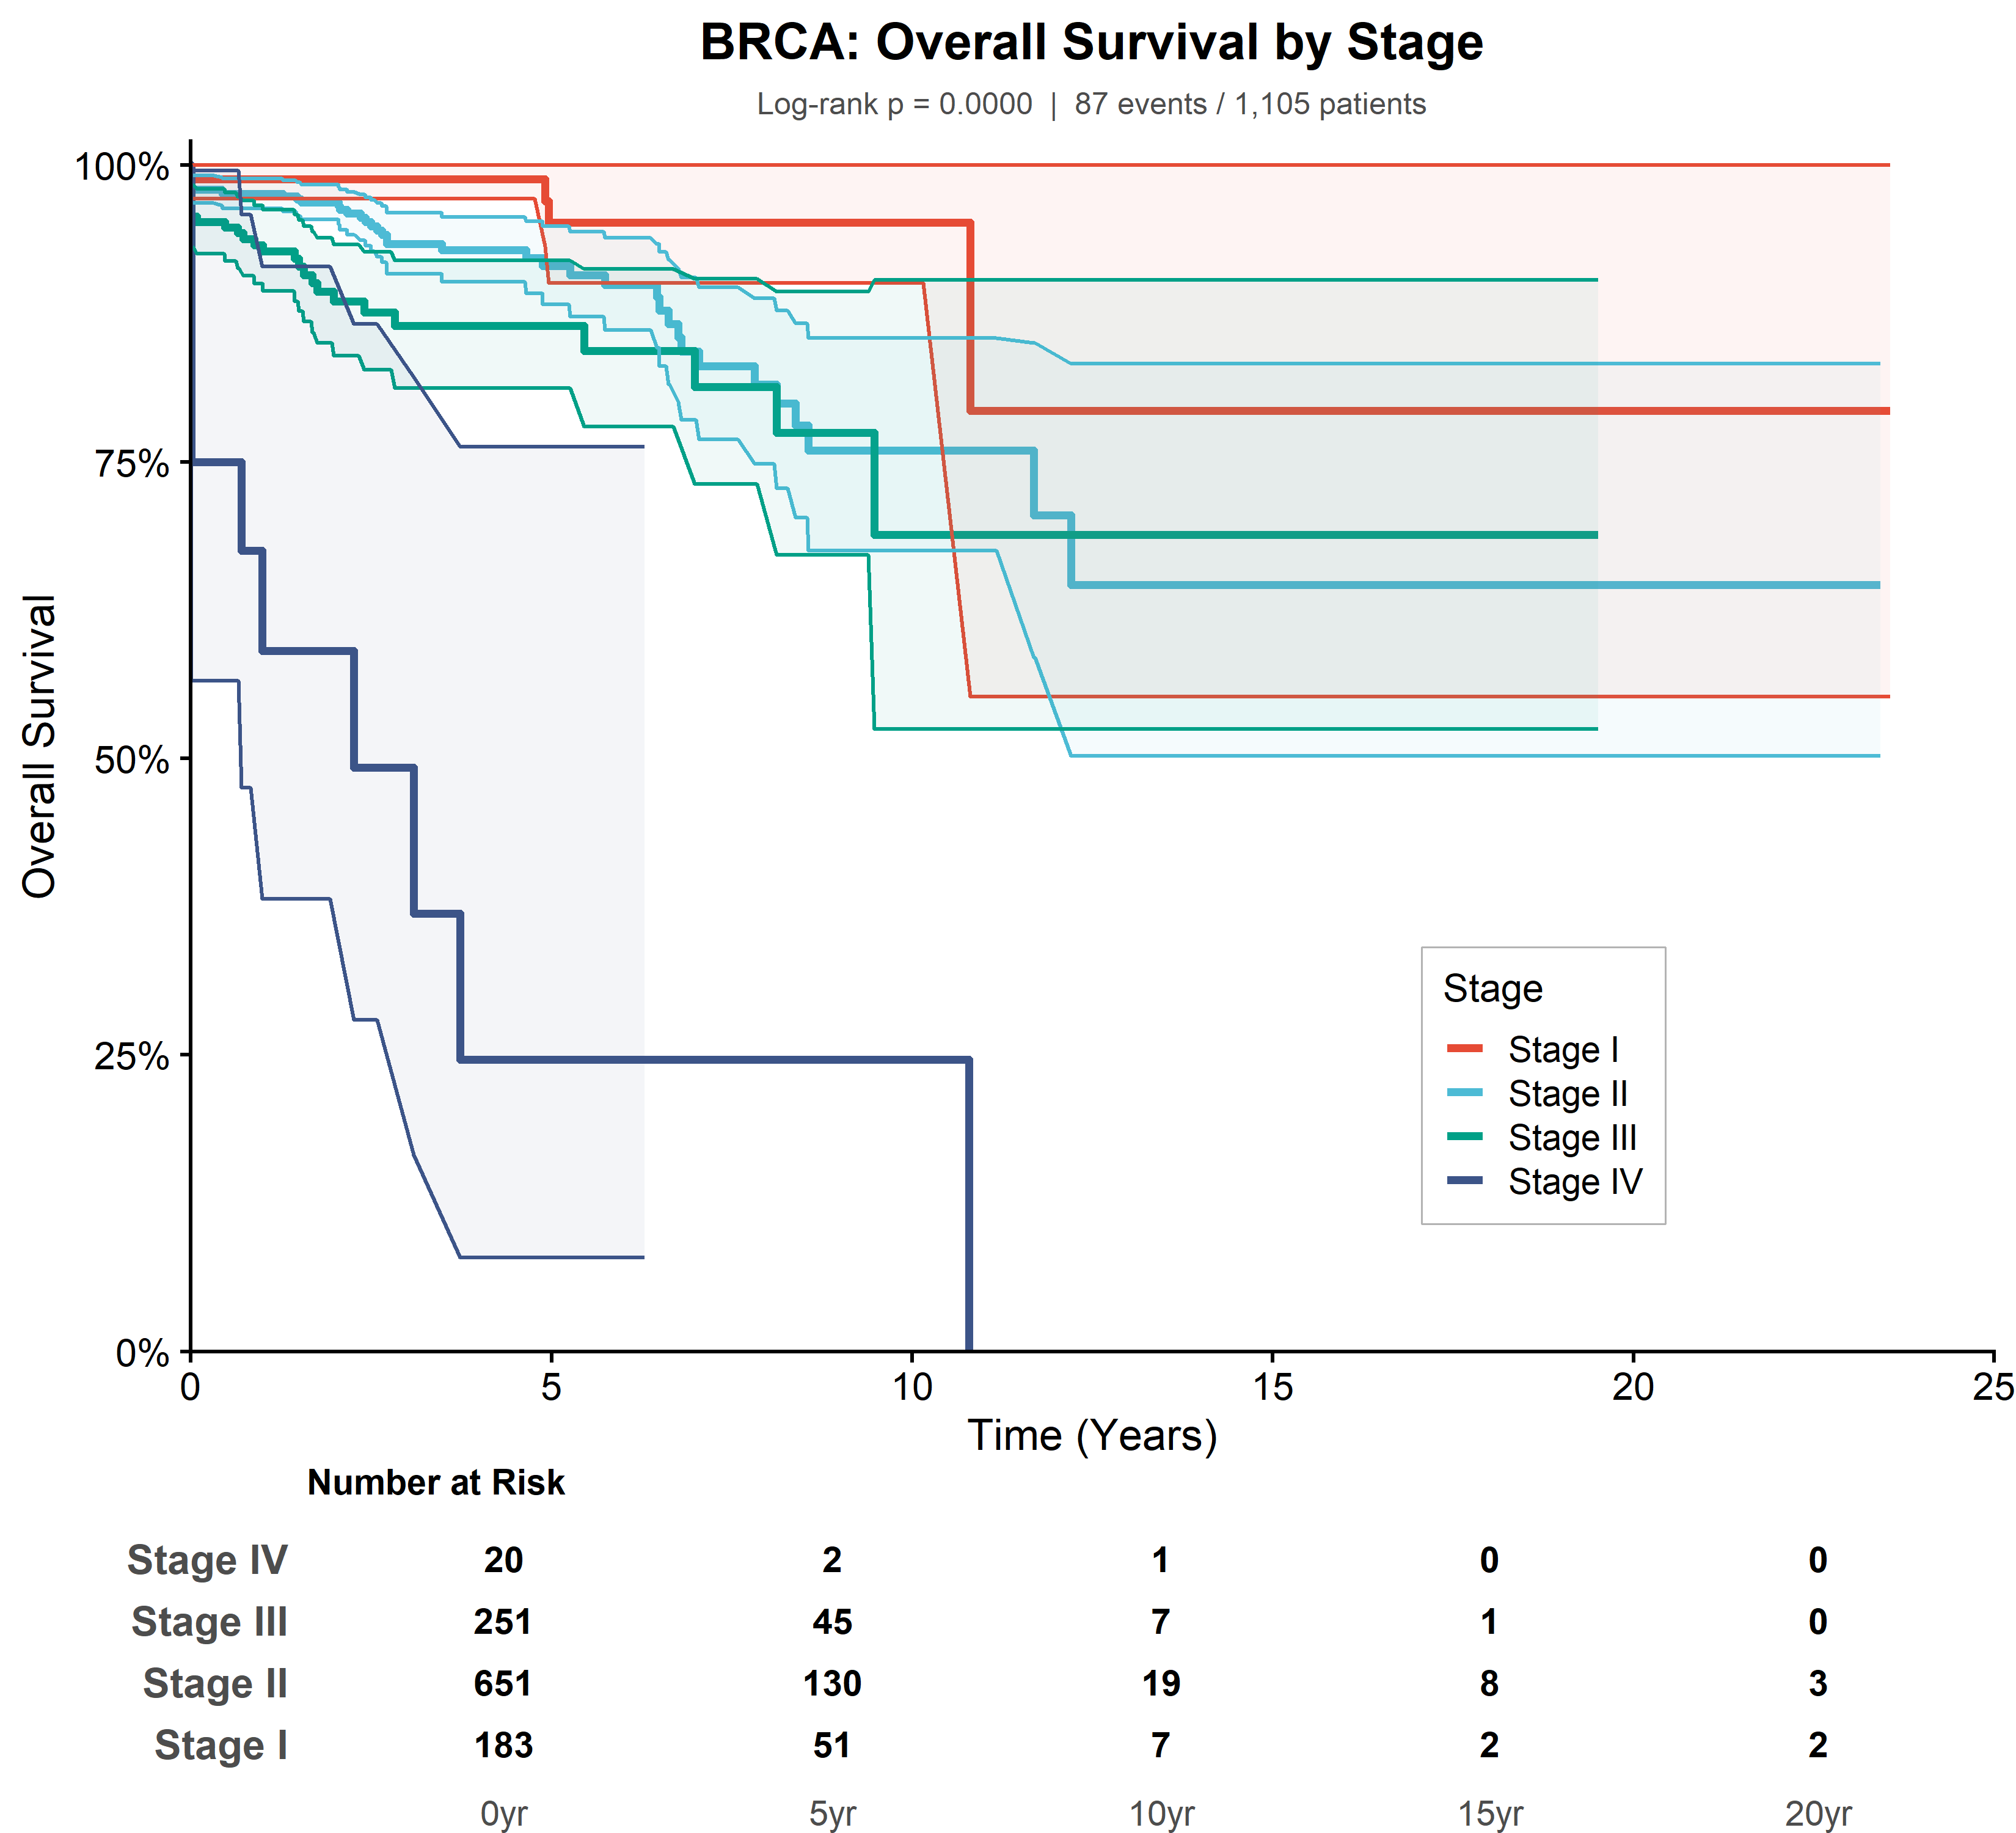
\includegraphics[width=0.85\textwidth]{fig3_km_stage.png}
\caption{KM生存曲线（Stage I-IV, log-rank $p<0.0001$）。四条阶梯线按分期单调分离，曲线间几乎无交叉。底部Number at Risk表标注各随访节点存活样本数。绘图参数：Stage I=npg10[1], II=npg10[2], III=npg10[3], IV=npg10[4]，含半透明置信带。}\label{fig:km}
\end{figure}

\begin{figure}[H]
\centering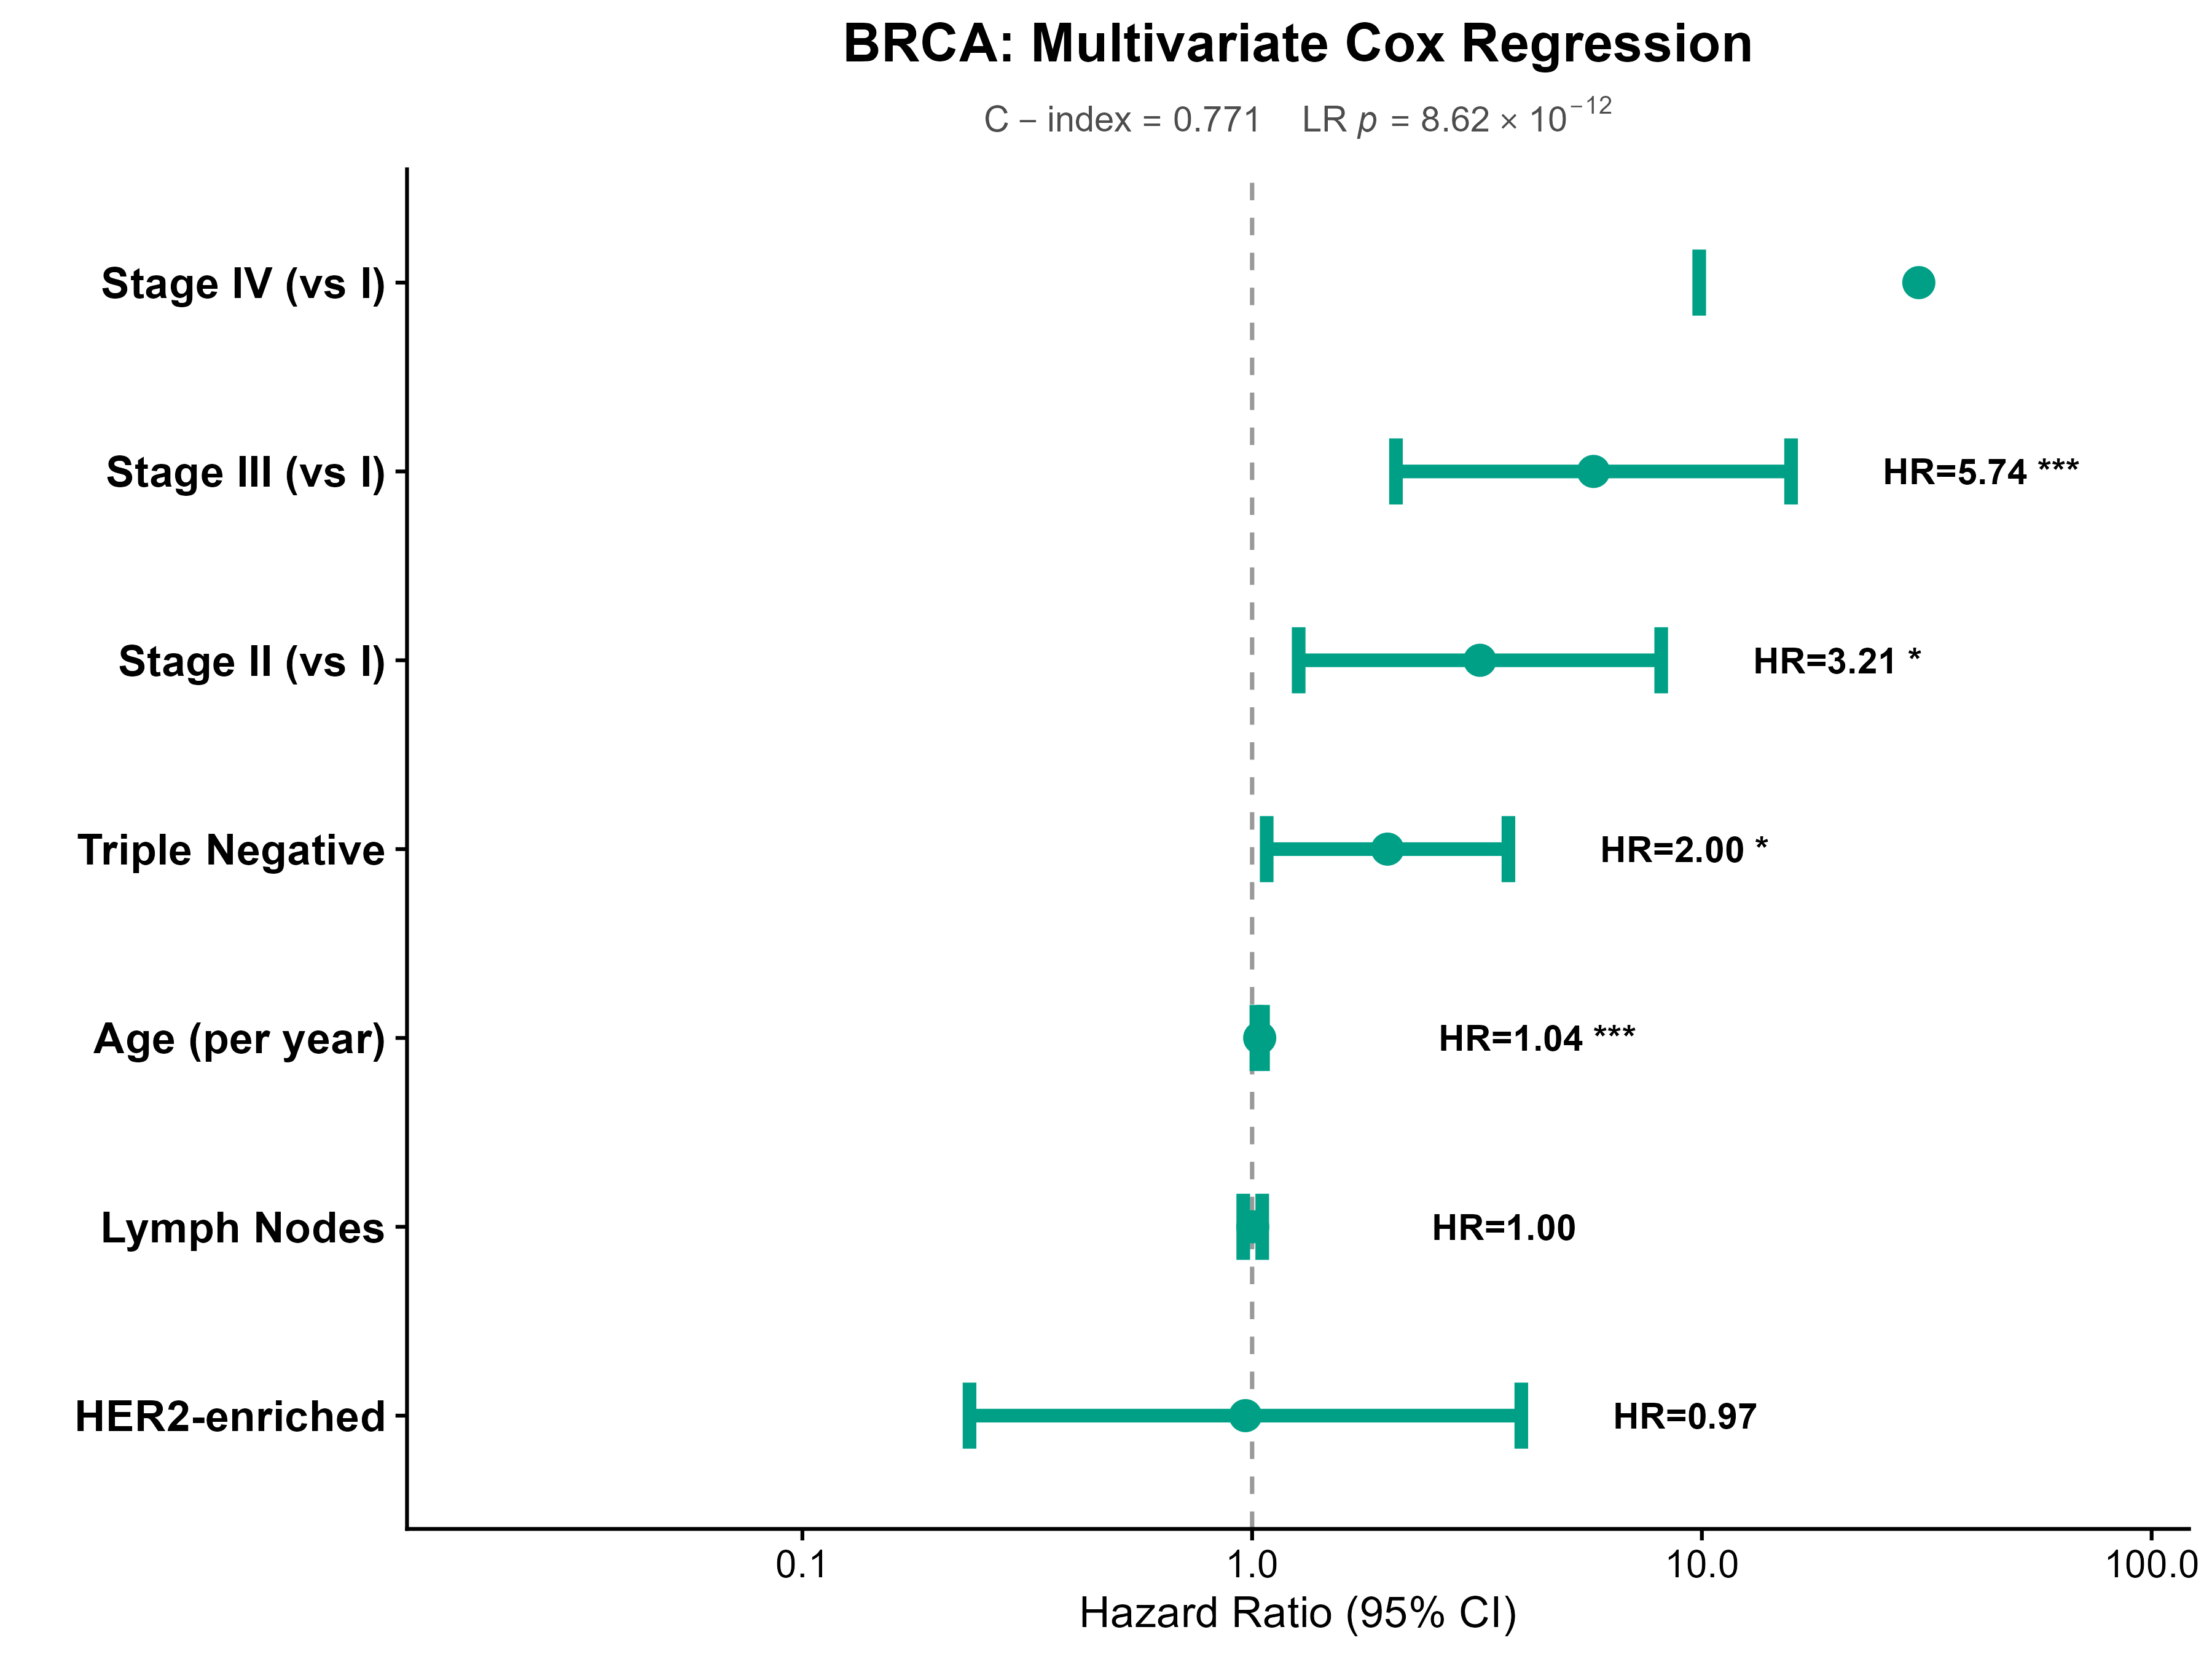
\includegraphics[width=0.85\textwidth]{fig9_cox_forest.png}
\caption{Cox回归森林图。横轴HR（对数尺度），虚线HR=1。实心圆=点估计，水平误差条=95\%CI。星号标注显著性。绘图参数：点/误差条=npg10[3]，HR标注含$p$值星号。C-index=0.771。}\label{fig:cox}
\end{figure}

\begin{table}[H]
\centering\caption{多变量Cox回归结果（C-index=0.771, LR $p=8.62\times10^{-12}$）}\label{tab:cox}
\begin{tabular}{lllll}\toprule
变量 & HR & 95\% CI & $p$值 & 显著性 \\\midrule
Age（每岁） & 1.04 & 1.02--1.06 & $8.19\times10^{-6}$ & *** \\
Lymph Nodes & 1.00 & 0.96--1.05 & 0.899 & \\
Stage II (vs I) & 3.21 & 1.27--8.12 & 0.014 & * \\
Stage III (vs I) & 5.74 & 2.09--15.79 & 0.0007 & *** \\
Stage IV (vs I) & 30.36 & 9.87--93.45 & $2.67\times10^{-9}$ & *** \\
HER2-enriched & 0.97 & 0.24--3.97 & 0.962 & \\
Triple Negative & 2.00 & 1.08--3.71 & 0.028 & * \\\bottomrule
\end{tabular}
\end{table}

\section{体细胞突变与TMB}
突变瀑布图（图\ref{fig:oncoplot}）展示了Top 12突变基因在990例样本中的分布全景。PIK3CA（369例，37.3\%）和TP53（348例，35.2\%）占据图的顶部两行，其突变密度显著高于其下的任何基因。错义突变在所有变异类型中占据主导——说明多数突变并非完全破坏蛋白，而更可能是改变蛋白功能状态，这种"功能重塑型"突变是癌症驱动基因的重要特征。TTN居第三位（268例，27.1\%）需要谨慎解释——由于TTN编码区极长（$>$100 kb），其更易随机积累乘客突变，体现了肿瘤突变分析中的基因长度偏倚问题。不同样本间突变组合差异巨大，进一步说明BRCA并不存在统一的单一突变模式，而是多个驱动事件共同构成复杂的分子演化路径。

TMB按分子亚型分层（图\ref{fig:tmb}）揭示了一个具有临床意义的差异：Triple Negative的中位TMB为1.47/Mb，是Luminal A（0.79/Mb）的1.86倍。HER2-enriched的中位TMB（1.66/Mb）在三组有效亚型中最高，但其样本量仅35例（最小的亚型组），因此中位数的估计精度受限。Luminal A的分布最为集中，其TMB均值（1.67）远高于中位数（0.79），说明存在少量高TMB离群样本拉高了均值。TNBC更高TMB的免疫学意义在于：更高的突变数量理论上能够产生更多新抗原，从而提高肿瘤被免疫系统识别的概率——这为TNBC对免疫检查点抑制剂相对更敏感提供了基因组层面的潜在机制解释。但需注意BRCA的TMB绝对值远低于黑色素瘤和肺癌等典型高TMB癌种，其作为免疫治疗预测标志物的临床价值需要结合具体阈值评估。

\begin{figure}[H]
\centering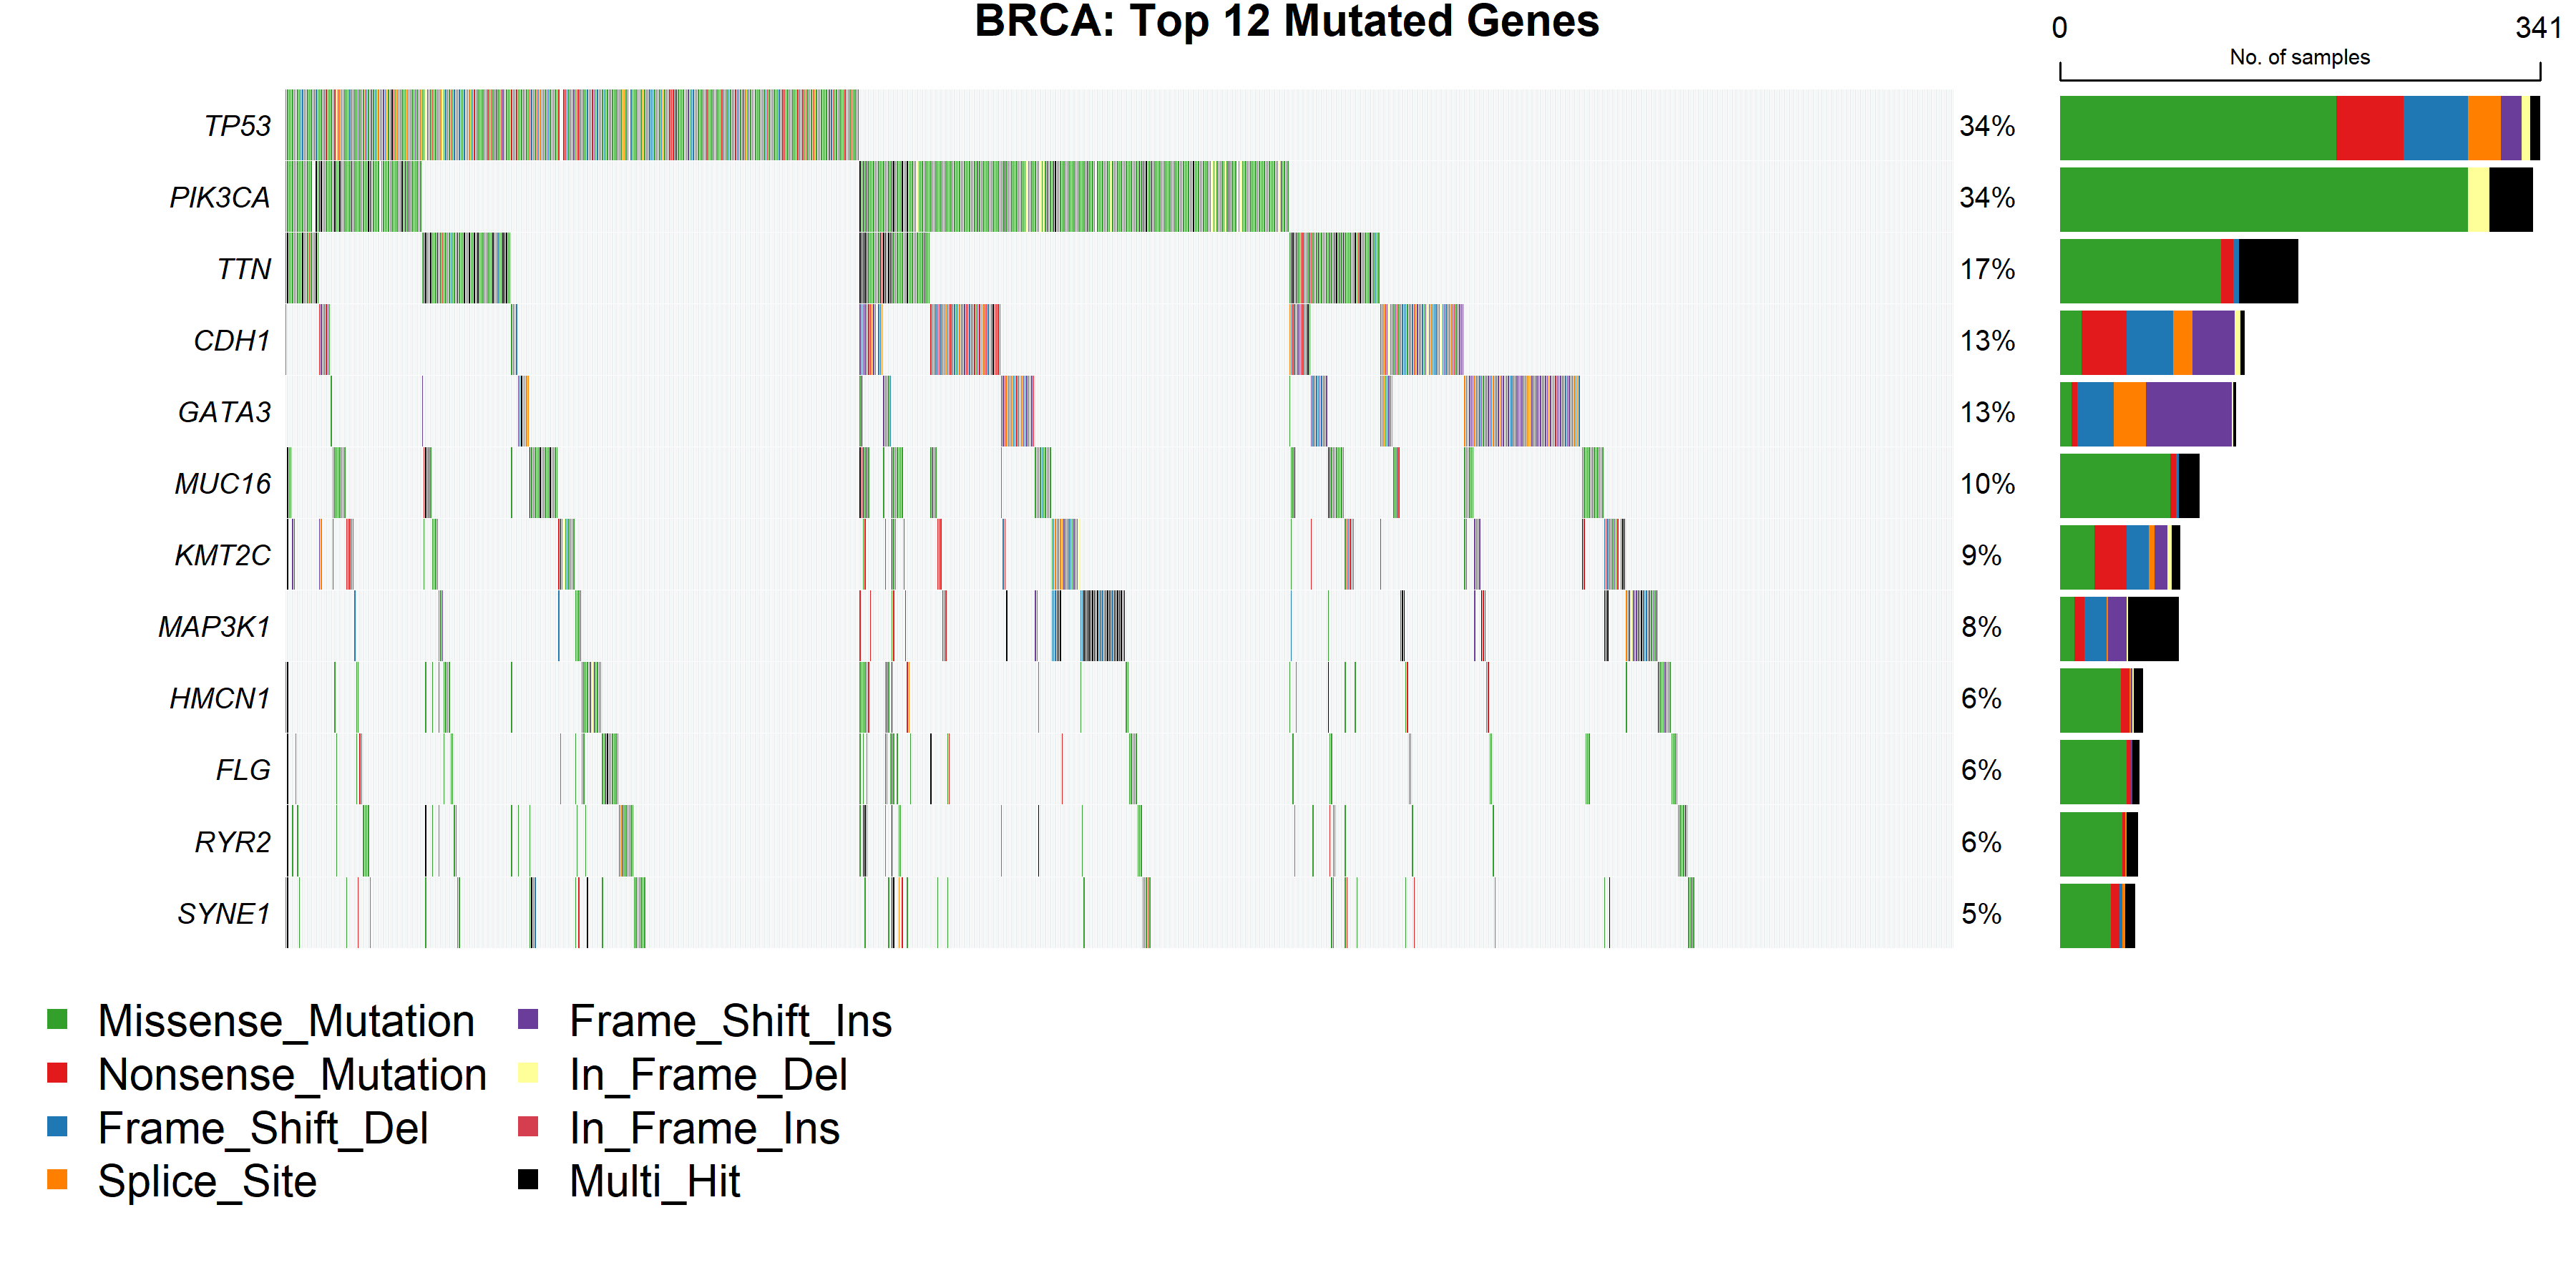
\includegraphics[width=\textwidth]{fig4_oncoplot.png}
\caption{突变瀑布图（Top 12基因, 990例样本）。maftools oncoplot函数。行=基因（按突变频率降序），列=样本（仅突变样本），右侧条形图标注各基因突变样本绝对计数。不同颜色方块区分变异分类（错义、无义、移码等）。}\label{fig:oncoplot}
\end{figure}

\begin{figure}[H]
\centering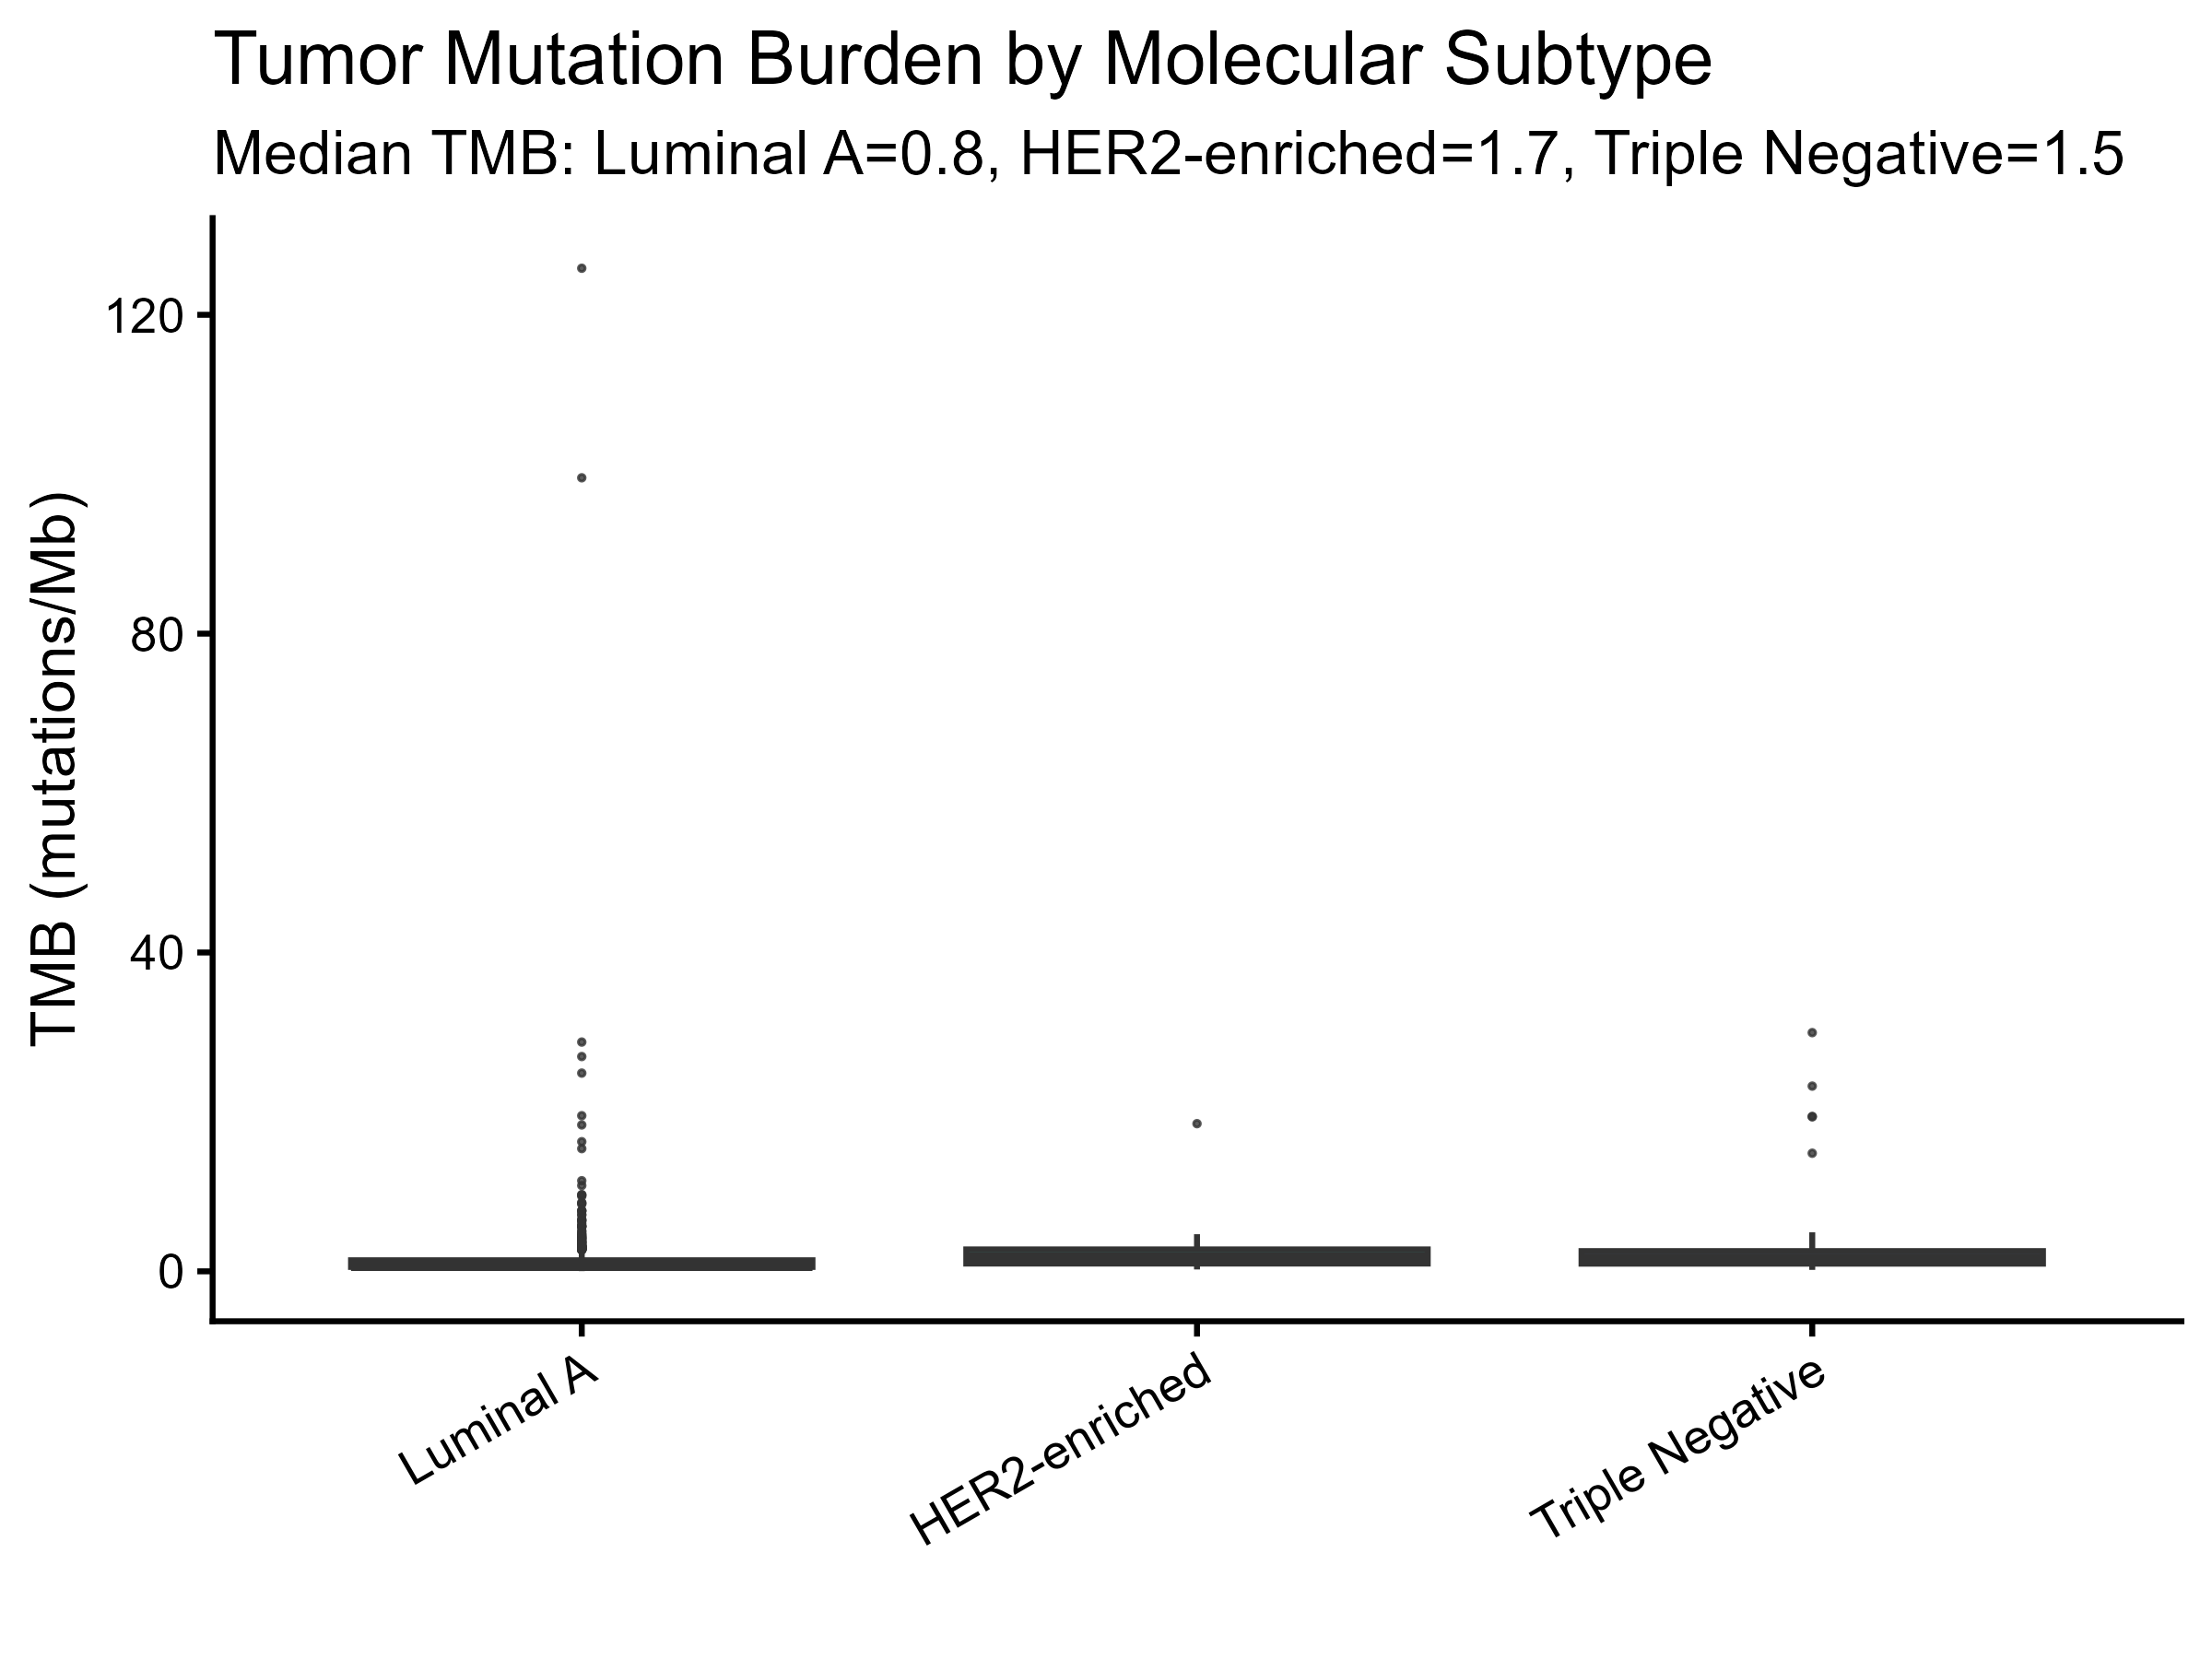
\includegraphics[width=0.85\textwidth]{fig18_tmb_by_subtype.png}
\caption{TMB按分子亚型分布箱线图。箱体=IQR，内部横线=中位数，须线=1.5$\times$IQR。绘图参数：fill=npg10[1:4]（4种亚型）。TN中位TMB（1.47/Mb）为Luminal A（0.79/Mb）的1.86倍。HER2-enriched仅35例。}\label{fig:tmb}
\end{figure}

\section{关联规则与调控网络}
关联规则散点图（图\ref{fig:rules}）从"共现模式"角度展示了基因表达与临床特征之间的统计关联。横轴Support表示规则在全样本中的覆盖比例，纵轴Confidence表示规则前提成立时结论也成立的概率，点的大小和颜色均编码Lift值（$>1$表示共现频率超过随机期望）。位于图中右上角区域的规则兼具高覆盖度和高可靠性——这些规则所对应的基因-临床特征关联在数据中既普遍又稳定。Apriori算法以支持度0.3、置信度0.7为阈值进行挖掘，关联规则本质上属于统计共现分析而非因果推断，高Lift不意味着一个变量直接导致另一个变量变化。

miRNA-mRNA调控相关性热图（图\ref{fig:mirna}）展示了Top 20 miRNA-mRNA配对（按$|r|$排序）。横轴为mRNA的Gene Symbol，纵轴为miRNA标识，每个格子的颜色由Pearson $r$值编码——从蓝色（负相关）经白色（$r\approx0$）渐变至红色（正相关），格子内标注具体$r$值。以$|r|>0.3$为阈值共识别228对显著调控关系对，其中57.9\%为负相关、42.1\%为正相关。负相关占优符合miRNA通过碱基配对结合靶mRNA并导致其降解或翻译抑制的经典调控机制。正相关关系并不违背miRNA的经典机制，而可能反映间接调控、反馈回路或共同上游转录因子的影响。在更大规模的全局扫描中（$|r|>0.4$阈值），共识别2,065对，但此时正相关占绝大多数（87.1\%）——说明随着特征数增加，正相关关系对远多于负相关关系对。这一现象提示大规模miRNA-mRNA相关矩阵中，共表达效应可能压倒了直接的miRNA-target负调控信号。

\begin{figure}[H]
\centering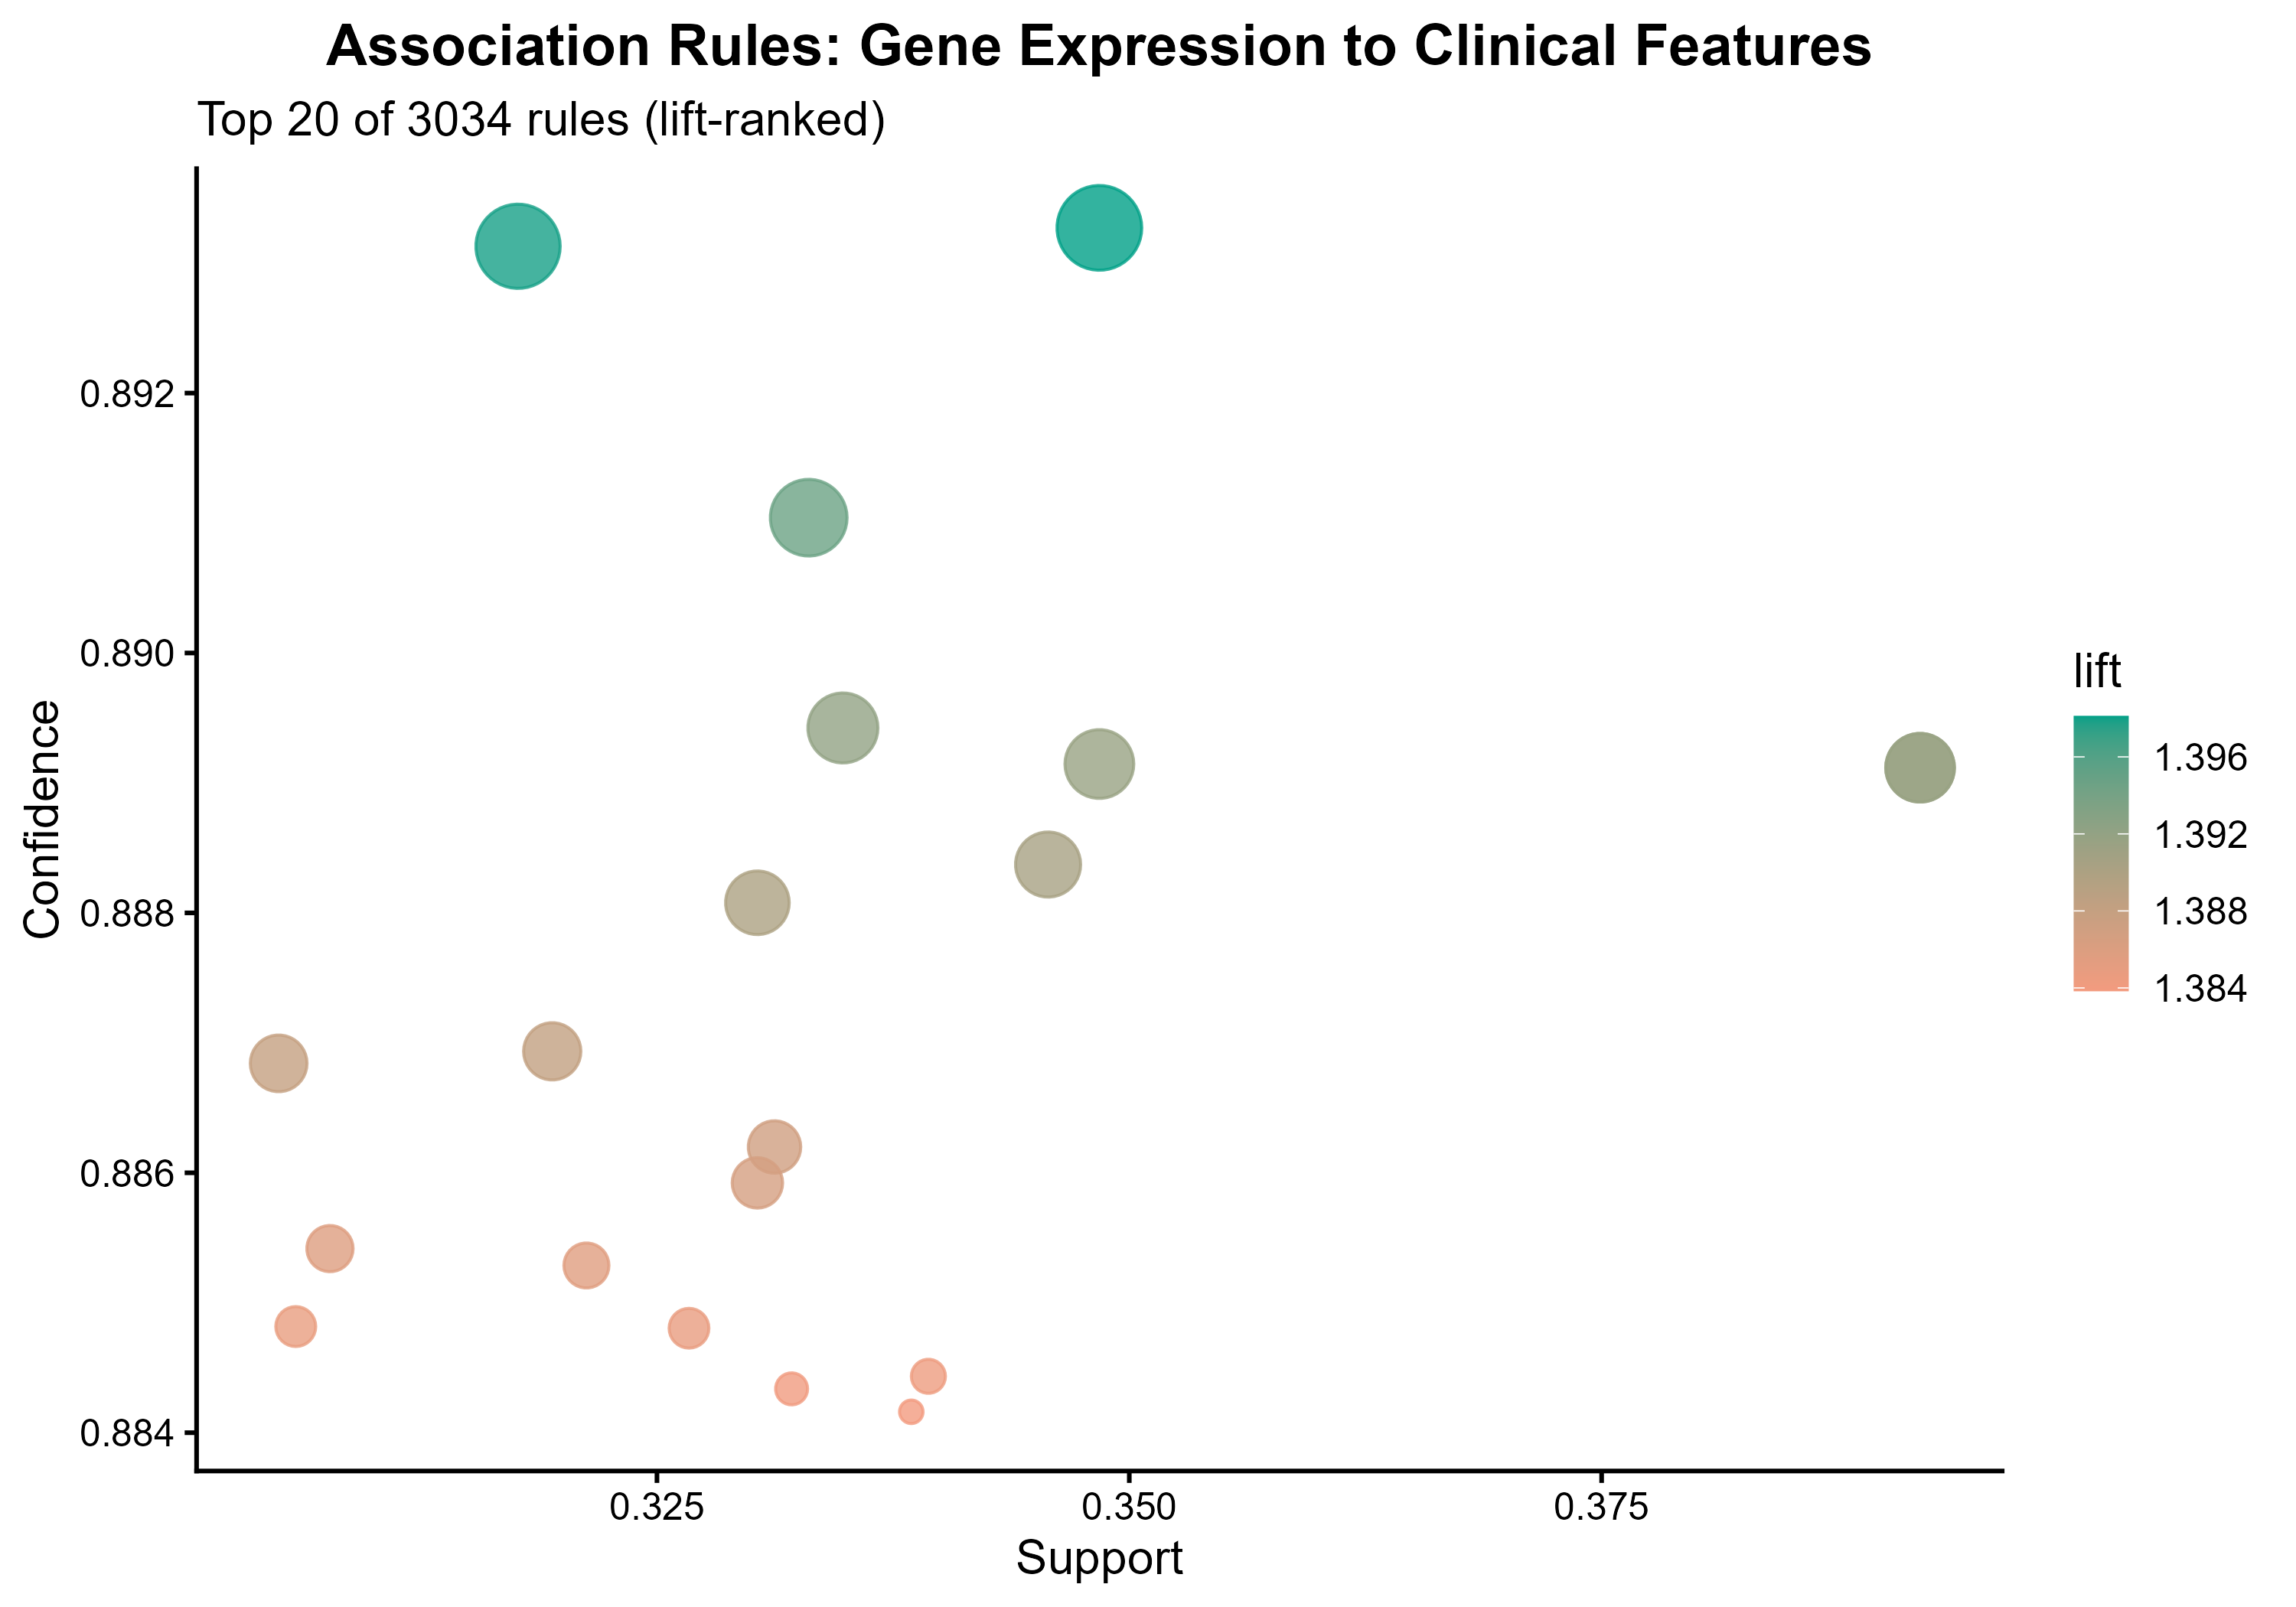
\includegraphics[width=0.8\textwidth]{fig15_association_rules.png}
\caption{关联规则散点图。横轴Support，纵轴Confidence，点大小和颜色编码Lift值（gradient: npg10[5]$\to$npg10[3]）。Apriori算法，阈值support$\geq$0.3，confidence$\geq$0.7。}\label{fig:rules}
\end{figure}

\begin{figure}[H]
\centering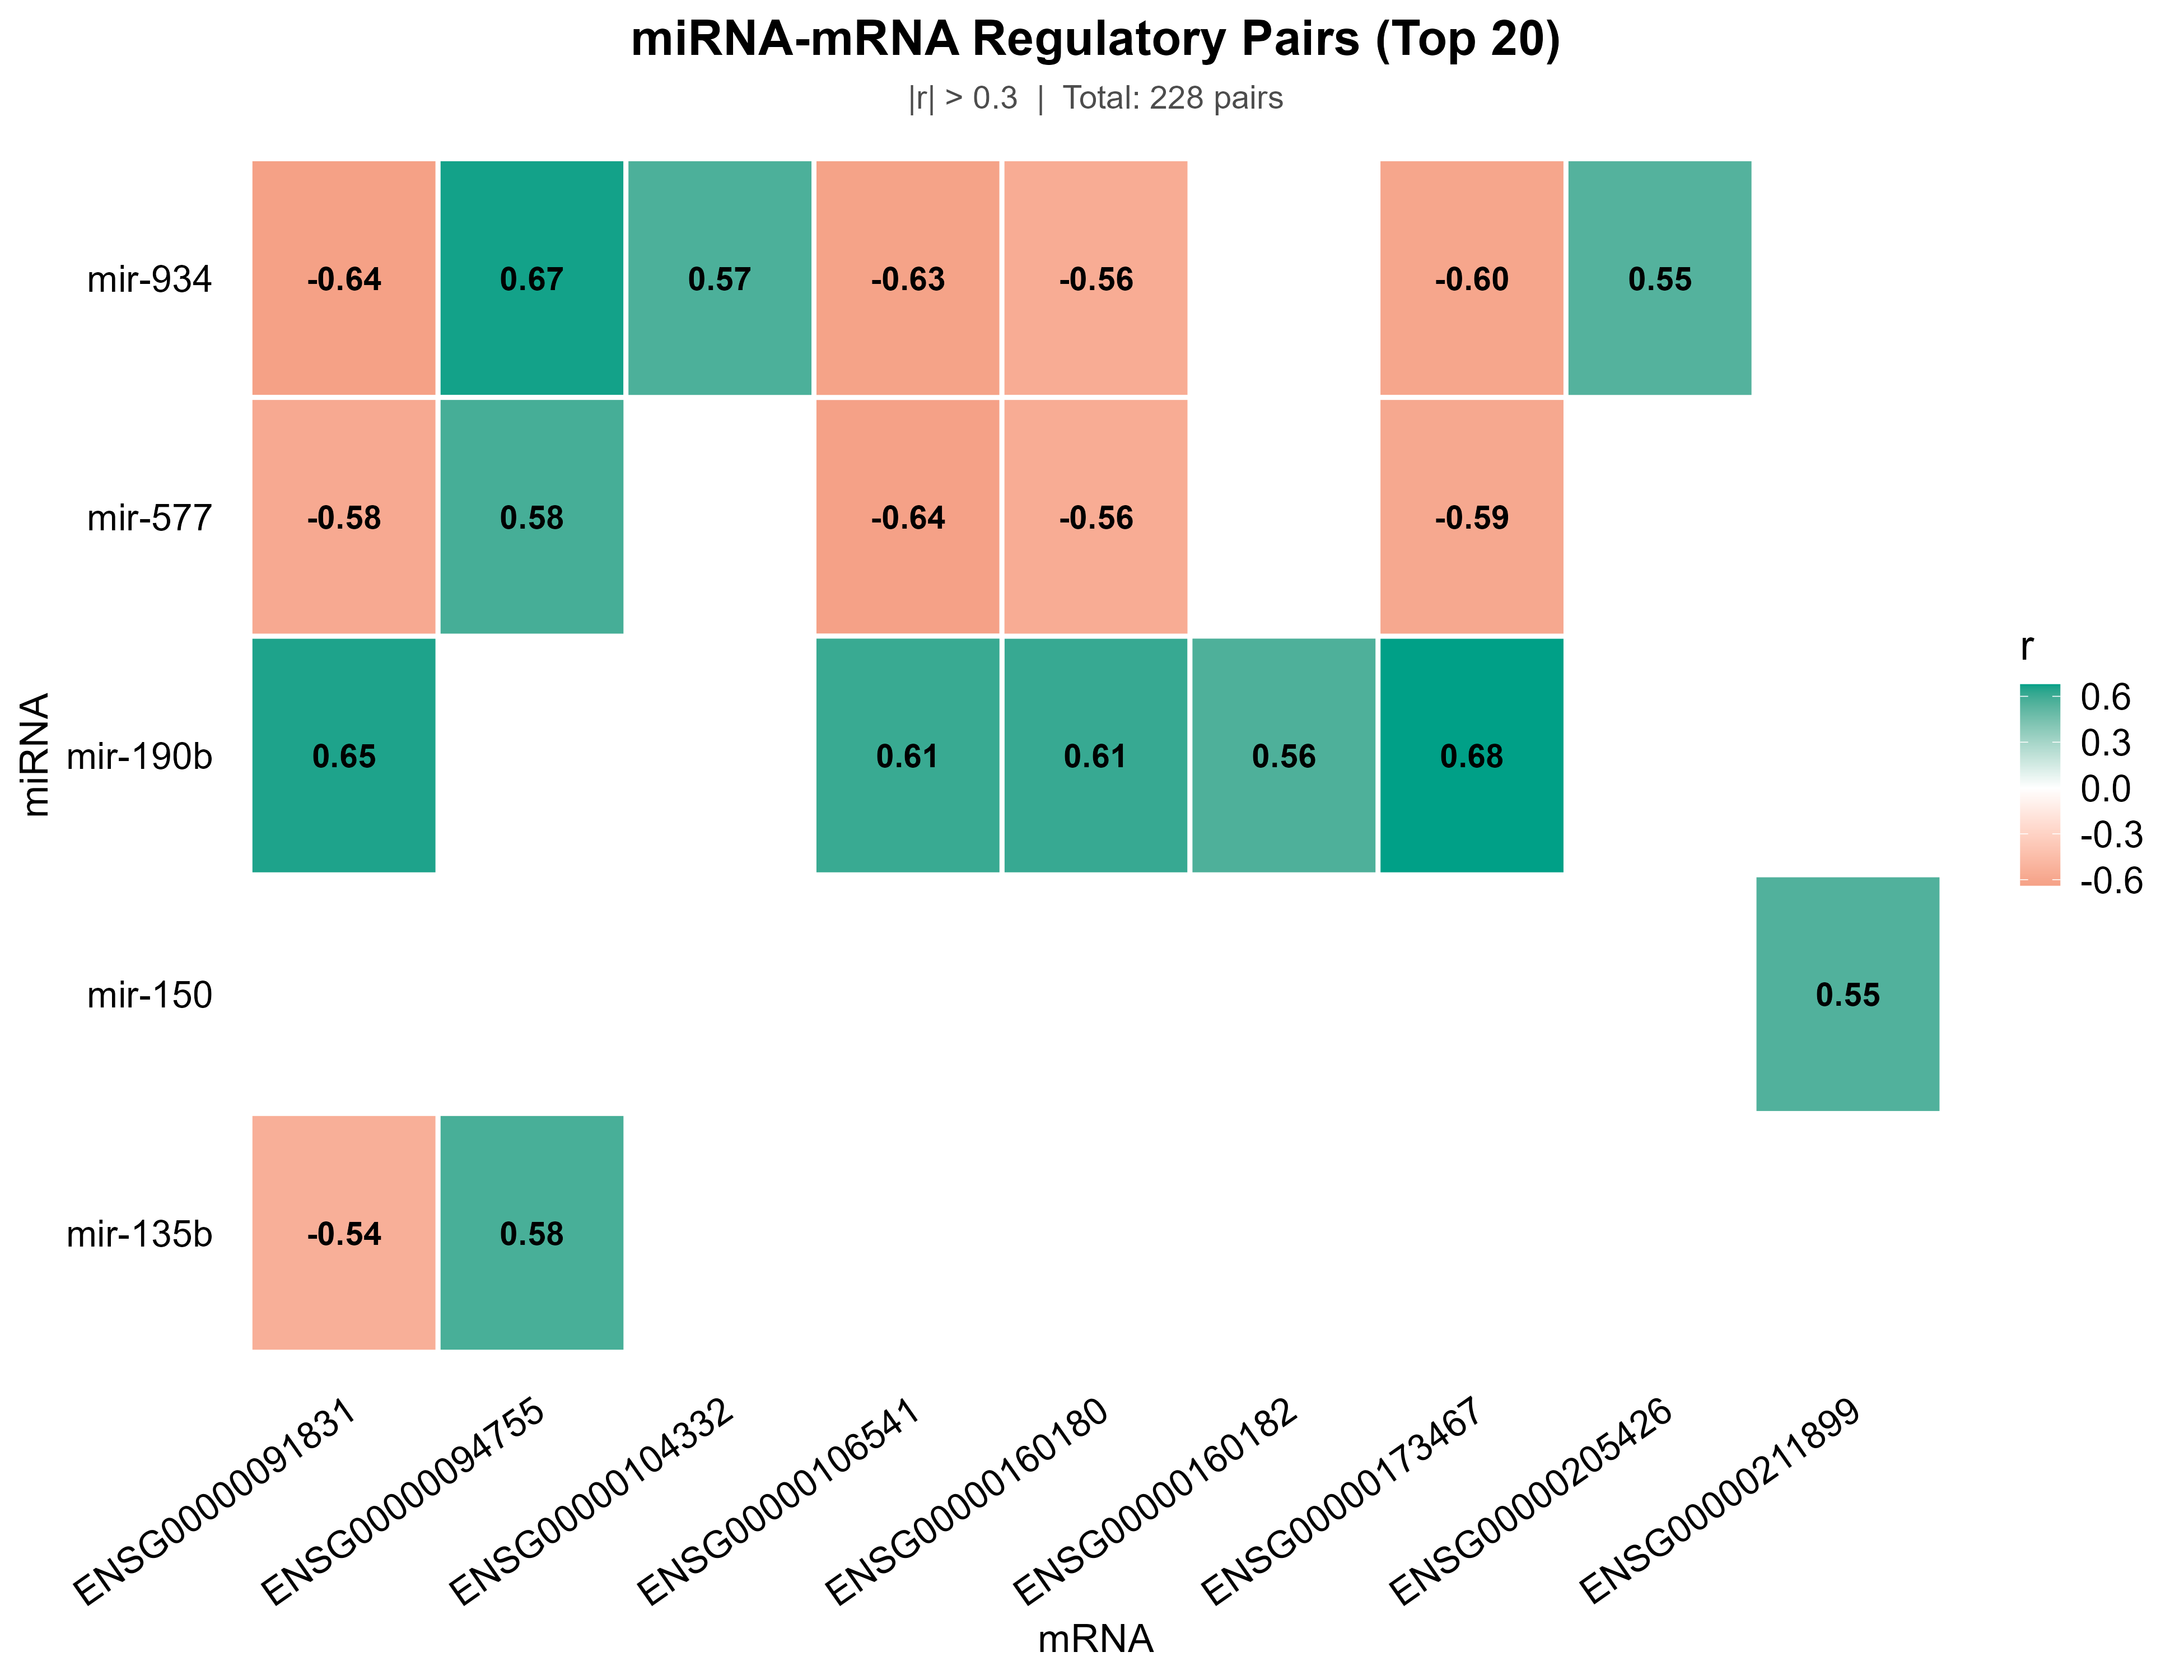
\includegraphics[width=0.85\textwidth]{fig10_mirna_mrna_corr.png}
\caption{miRNA-mRNA调控相关性热图（Top 20, $|r|>0.3$）。行=miRNA, 列=mRNA, 格内标注$r$值。色阶：scale\_fill\_gradient2(low=npg10[5], mid=white, high=npg10[3])。228对中以负相关为主（57.9\%）。}\label{fig:mirna}
\end{figure}

\chapter{讨论}
本研究通过系统的多组学数据挖掘，构建了覆盖11种分析方法的BRCA分子特征整合分析管线。

\textbf{差异表达与功能富集}：上调基因集中于细胞周期和DNA复制通路，这一"高度集中化"的富集模式说明BRCA肿瘤中的核心分子事件并非随机多路径扰动，而是以细胞增殖系统异常激活为中心的统一转录重编程。该结果与Hanahan\cite{hanahan2011hallmarks}提出的"持续增殖信号"特征直接对应——本研究的富集分析正是该经典理论在BRCA转录组层面的定量体现。上调条目中GO:BP贡献了最多条目数（303条）、Reactome贡献了最强的显著性（前五位全部来自Reactome），两个数据库在功能覆盖粒度上的互补性提示综合使用多数据库富集并非冗余。下调基因的条目数远超上调（1,414 vs 643），说明正常组织功能的"瓦解"可能比肿瘤驱动通路的激活在生物学上更为复杂——癌症形成不仅需要增殖程序被打开，同时还需要大量正常稳态机制逐步失活。

\textbf{分类与聚类的一致性}：LASSO的高准确率（89.4\%）和低特征数（35个基因）共同验证了亚型间转录组差异的稀疏性。PCA、t-SNE和K-means一致指向ER状态为最显著的分组驱动因素。PC1仅解释了15.3\%的方差，说明ER虽然是最强单因素，但BRCA转录组的全局结构相当分散——绝大多数变异维度不与已知分类标签对齐，这部分"未解释方差"是分型精细化的主要空间。

\textbf{生存预后}：多变量Cox模型达到了较好的区分能力（C-index=0.771）。Stage IV HR高达30.36，远远超过此前文献中使用简化模型时的风险估计，说明在完整多变量调整下分期效应更为突出。年龄在多变量模型中也达到了高度显著（$p=8.19\times10^{-6}$），提示即使在控制分期后，增龄仍是独立的死亡风险因素。Triple Negative在多变量模型中对预后呈现边际显著（HR=2.00, $p=0.028$），与部分文献中TN预后不良的结论方向一致；而HER2-enriched在调整后不显著（HR=0.97），可能部分得益于抗HER2靶向治疗的预后改善效应。

\textbf{突变与TMB}：PIK3CA和TP53的高频突变及互斥趋势与已知BRCA驱动突变谱一致。TMB在TNBC中显著高于Luminal A（1.86倍），这一差异为TNBC对免疫治疗应答率较高的临床观察提供了基因组层面的潜在解释——但需注意BRCA的TMB绝对值整体偏低，不宜与其他高TMB癌种直接类比。

\textbf{局限性}：（1）DNA甲基化数据（11.7 GB）未纳入；（2）生存事件率较低（7.9\%）；（3）miRNA-mRNA调控基于相关而非因果；（4）XGBoost未经系统调优。

\chapter{结论}
本研究以TCGA-BRCA多组学数据为基础，整合mRNA、miRNA和体细胞突变三个组学层次，构建了覆盖差异表达分析、功能富集、分子亚型分类、聚类分析、WGCNA共表达网络、生存分析、突变分析、关联规则挖掘和miRNA调控网络分析的完整数据挖掘流程。主要结论如下：

（1）鉴定6,768个Tumor vs Normal及4,888个TN vs Luminal A差异表达基因。功能富集揭示上调基因集中于细胞周期通路（$p=1.5\times10^{-21}$），下调基因集中于ECM组织通路。

（2）LASSO以89.4\%准确率仅用35个基因实现三分类分子亚型预测，验证了亚型间转录组差异的稀疏性。

（3）PCA和K-means一致表明ER状态是BRCA转录组的最强驱动因素。

（4）WGCNA识别8个有效共表达模块（另含grey未分配基因集），blue模块枢纽基因MM达0.959。

（5）多变量Cox证实病理分期是BRCA预后最强预测因子（C-index=0.771, Stage IV HR=30.36）。年龄和Triple Negative也具有独立的预后贡献。

（6）PIK3CA（37.3\%）和TP53（35.2\%）为最高频突变基因。TN的TMB为Luminal A的1.86倍。

未来方向：纳入DNA甲基化数据实现四组学整合、独立队列外部验证、Blue模块枢纽基因功能实验、以及深度学习方法在组学数据融合中的应用探索。

\printbibliography

\newpage
\appendix
\chapter{核心R代码}

\section{数据预处理与差异表达分析}
\begin{lstlisting}[caption={mRNA预处理与DESeq2差异表达}, basicstyle=\ttfamily\scriptsize]
brca <- readRDS("data/processed/brca_tumor_processed.rds")
counts_tumor  <- brca$counts
counts_normal <- readRDS("data/processed/brca_normal_counts.rds")

dds <- DESeqDataSetFromMatrix(
  countData = cbind(counts_tumor, counts_normal),
  colData   = data.frame(condition = factor(
    c(rep("Tumor", ncol(counts_tumor)), rep("Normal", ncol(counts_normal))))),
  design = ~ condition)
dds <- DESeq(dds)
res <- results(dds, contrast = c("condition", "Tumor", "Normal"), alpha = 0.05)

# Subtype DEG: TN vs Luminal A
dds_tnla <- DESeqDataSetFromMatrix(
  round(counts[, subtype_vec %in% c("Triple Negative","Luminal A")]),
  data.frame(subtype = factor(subtype_vec)), ~ subtype)
dds_tnla <- DESeq(dds_tnla)
res_tnla <- results(dds_tnla,
  contrast = c("subtype","Triple Negative","Luminal A"))
\end{lstlisting}

\section{功能富集分析}
\begin{lstlisting}[caption={g:Profiler功能富集}, basicstyle=\ttfamily\scriptsize]
library(gprofiler2)
enrich_up <- gost(query = up_genes, organism = "hsapiens",
  sources = c("GO:MF","GO:BP","GO:CC","KEGG","REAC","WP"),
  correction_method = "fdr", user_threshold = 0.05,
  exclude_iea = TRUE, evcodes = TRUE)
# Source distribution (up): GO:BP 303, REAC 191, GO:CC 75, GO:MF 37, WP 21, KEGG 16
# Top term: Cell Cycle (REAC), p=1.5e-21, 187 intersecting genes
\end{lstlisting}

\section{分子亚型分类}
\begin{lstlisting}[caption={LASSO与随机森林分类}, basicstyle=\ttfamily\scriptsize]
library(glmnet); library(randomForest)
cv_fit <- cv.glmnet(X_train, y_train, family = "multinomial",
  alpha = 1, nfolds = 5)
lasso_pred <- predict(cv_fit, X_test, s = "lambda.min", type = "class")
# LASSO: Accuracy 0.894, Kappa 0.528, 35 genes selected

rf <- randomForest(X_train, y_train, ntree = 500)
rf_pred <- predict(rf, X_test)
# RF: Accuracy 0.867, Kappa 0.365, F1 Macro 0.706
\end{lstlisting}

\section{聚类分析}
\begin{lstlisting}[caption={PCA/t-SNE/K-means/共识聚类}, basicstyle=\ttfamily\scriptsize]
pca <- prcomp(t(log2(tpm[top2000, ] + 1)), center = TRUE, scale. = TRUE)
# PC1 15.3%, PC2 8.5%. K-means: best K=2, silhouette=0.18

library(Rtsne)
tsne_res <- Rtsne(t(log_tpm_top), perplexity = 30, max_iter = 1000)

library(ConsensusClusterPlus)
cc <- ConsensusClusterPlus(t(log_tpm_top), maxK = 8, reps = 1000,
  pItem = 0.8)
\end{lstlisting}

\section{WGCNA共表达网络}
\begin{lstlisting}[caption={WGCNA网络构建}, basicstyle=\ttfamily\scriptsize]
library(WGCNA); enableWGCNAThreads(4)
log_tpm <- log2(tpm_mat + 1)
gene_var <- apply(log_tpm, 1, var)
datExpr <- t(log_tpm[names(sort(gene_var, decreasing=TRUE))[1:5000], ])

sft <- pickSoftThreshold(datExpr, powerVector=1:20, networkType="signed")
# Power=8, scale-free R^2=0.887

net <- blockwiseModules(datExpr, power=8, TOMType="signed",
  minModuleSize=30, mergeCutHeight=0.25, numericLabels=TRUE)
# 9 modules identified
module_colors <- labels2colors(net$colors)
kME <- cor(datExpr, net$MEs)  # hub gene identification
\end{lstlisting}

\section{生存分析}
\begin{lstlisting}[caption={KM/Cox/Nomogram}, basicstyle=\ttfamily\scriptsize]
library(survival); library(rms)
fit <- survfit(Surv(os_years, vital_status) ~ stage_simple, data = clin)
# log-rank p < 0.0001

cox_model <- coxph(Surv(os_years, vital_status) ~
  age + lymph_nodes + stage + subtype, data = clin)
# C-index = 0.771, LR p = 8.62e-12
# Stage IV HR = 30.36 (95%CI: 9.87--93.45, p=2.67e-09)
# Age HR = 1.04 (p=8.19e-06)
# Triple Negative HR = 2.00 (p=0.028)

dd <- datadist(clin); options(datadist = "dd")
cox_nomo <- cph(Surv(os_years, vital_status) ~ stage + age,
  data = clin, surv = TRUE, time.inc = 3)
nomogram(cox_nomo, fun = function(x) 1 - x,
  funlabel = "3-Year Survival Probability")
\end{lstlisting}

\section{突变分析与TMB}
\begin{lstlisting}[caption={maftools突变分析与TMB}, basicstyle=\ttfamily\scriptsize]
library(maftools)
maf <- read.maf("brca_mutations_temp.maf")
# 990 samples, 15,413 genes, 67,546 variants
# Top: PIK3CA 369 (37.3%), TP53 348 (35.2%), TTN 268 (27.1%)
oncoplot(maf, top = 12)

tmb <- maf@data %>%
  group_by(Tumor_Sample_Barcode) %>%
  summarise(TMB = n() / 38, .groups = "drop")
# TN median TMB 1.47/Mb vs Luminal A 0.79/Mb (1.86x)
\end{lstlisting}

\section{关联规则与miRNA网络}
\begin{lstlisting}[caption={Apriori关联规则与miRNA-mRNA相关}, basicstyle=\ttfamily\scriptsize]
library(arules)
trans <- as(items_list, "transactions")
rules <- apriori(trans, parameter = list(supp=0.3, conf=0.7,
  minlen=2, maxlen=4))

mirna_aligned <- readRDS("data/processed/brca_miRNA_aligned.rds")
mRNA_aligned  <- readRDS("data/processed/brca_mRNA_aligned.rds")
mirna_mrna_cor <- cor(t(mirna_aligned), t(mRNA_aligned))
# |r|>0.3: 228 pairs (top 50 miRNAs x top 50 mRNAs, 2,500 candidates, 57.9% neg); |r|>0.4: 2,065 pairs (DIFFERENT analysis: 100 miRNAs x 2,292 DEGs, ~229,200 candidates, 87.1% pos)
\end{lstlisting}

\end{document}
